% $Id:$

\documentclass{cmspaper}
\input epsf
\usepackage{graphicx}
%==========================================================
\usepackage{epic,rotating,epsfig}
\usepackage{amssymb}
\usepackage{amsmath}
\usepackage{pstricks,pst-grad}
%
% Units
%
\def\cm{\hbox{$\;\hbox{\rm cm}$}}
%
%newcommand{\TeVcc}{\ensuremath{\,\mathrm{Te\kern -0.1em V\!/c}^2}}
%\newcommand{\GeVcc}{\ensuremath{\,\mathrm{Ge\kern -0.1em V\!/c}^2}}
%\newcommand{\MeVcc}{\ensuremath{\,\mathrm{Me\kern -0.1em V\!/c}^2}}
%\newcommand{\GeVc}{\ensuremath{\mathrm{Ge\kern -0.1em V}\!/c}}
%
\newcommand{\GeV}{\ensuremath{\mathrm{Ge\kern -0.1em V}}}
\newcommand{\TeVcc}{\ensuremath{\,\mathrm{Te\kern -0.1em V\!/c}^2}}
\newcommand{\GeVcc}{\ensuremath{\,\mathrm{Ge\kern -0.1em V\!/c}^2}}
\newcommand{\MeVcc}{\ensuremath{\,\mathrm{Me\kern -0.1em V\!/c}^2}}
\newcommand{\GeVc}{\ensuremath{\mathrm{Ge\kern -0.1em V}\!/c}}
\newcommand{\nanob}{\mbox{{\rm ~nb}~}}
\newcommand{\fb}{\ensuremath{\mathrm{fb}}}
\newcommand{\pb}{\ensuremath{\mathrm{pb}}}
\newcommand{\ifb}{\ensuremath{\mathrm{fb^{-1}}}}
\newcommand{\ipb}{\ensuremath{\mathrm{pb^{-1}}}}
%
% Special user made math symbols
%
\newcommand{\lsim}{\raisebox{-1.5mm}{$\:\stackrel{\textstyle{<}}{\textstyle{\sim}}\:$}}
\newcommand{\gsim}{\raisebox{-1.5mm}{$\:\stackrel{\textstyle{>}}{\textstyle{\sim}}\:$}}
%
%==========================================================
\begin{document}

%==============================================================================
% title page for few authors

\begin{titlepage}

% select one of the following and type in the proper number:
%  \cmsnote{2005/000}
 % \internalnote{2007/000}
%  \conferencereport{2005/000}
   %\date{7 November 2007}
   \date{\today}

  \title{Review Documentation for the\\ CMS Storage Manager}

  \begin{Authlist}
    W.~Badgett, K.~Biery, H.~Cheung, J.~Kowalkowski, 
    E.~Sexton-Kennedy, D.~Shpakov
       \Instfoot{fermilab}{Fermilab, Batavia, IL, USA}
    G.Bauer, C.~Loizides, C.~Paus, M. Rudolph 
       \Instfoot{mit}{MIT, Cambridge, MA, USA}
  \end{Authlist}

% if needed, use the following:
\collaboration{Storage Manager Working Group}
%\collaboration{CMS collaboration}


  \begin{abstract}
The CMS Storage Manager system is designed to store raw data on a storage medium close to the
experiment, give real-time access to a fraction of the collected data for monitoring purposes, and
collect non-event monitoring data. The design specifications for the system are a total storage capacity
of 250 TB and a maximum throughput of 1 GB/s. This note presents the hardware and software
architecture of  the Storage Manager system, describes future upgrade plans and operational 
needs are discussed. 
  \end{abstract} 

% if needed, use the following:
%\conference{Presented at {\it Physics Rumours}, Coconut Island, April 1, 2005}
%\submitted{Submitted to {\it Physics Rumours}}
%\note{Working version}
  
\end{titlepage}

\setcounter{page}{2}%JPP
%==============================================================================

% $Id: introduction.tex,v 1.4 2008/05/26 20:01:03 gbauer Exp $

\section{\label{sec:intro}Introduction}

The Large Hadron Collider (LHC) at CERN is scheduled to begin operation in 2008 
and will deliver proton-proton collisions to the CMS detector at a center-of-mass energy 
of up to 14~TeV and a crossing rate of 40~MHz. 
This rate must be reduced significantly to comply with the limitations of the computing resources to process the collected data for physics analysis. 
At the same time interesting physics signals must be triggered with high efficiency. 
CMS uses a two level trigger system to reduce the rate to approximately 100~Hz. 
The Level-1 trigger is based on custom hardware and designed to reduce the rate to about 100~kHz, corresponding to 100~GB/s, assuming an average event size of 1~MB. 
The High Level Trigger (HLT) is purely software-based and  must achieve the remaining data reduction by executing quality algorithms with an average event processing time of 40~ms. 
Events accepted by the HLT are send to the Storage Manager system, where they are organized in streams according to the specific physics content as identified by the HLT filter decision. 
The HLT output rate is nominally expected to be 100-300~Hz and the event size 1-2.5~MB. 
We therefore designed a system which is able to handle 1~GB/s throughput with a buffer of 3 days, 
equivalent to 250~TB.
Beside collecting event data, the Storage Manager is responsible for collection of Data Quality Monitoring (DQM) information produced in the HLT. 
Events and DQM information are written to disk and a fraction of the information can be served to consumer clients. 
The raw data files on disk are then moved to the Tier-0 computing center for further processing. 

The primary functions of the Storage Manager are the following:
\begin{itemize}
\item Receive events from HLT,
\item Write events to disks at up to 1~GB/s (baseline),
\item Transport files to the Tier-0 at up to 1~GB/s,
\item Buffer data to up to 3 days,
\item Serve events and monitoring elements to online monitoring clients,
\end{itemize}

Recently, however, CMS management has recently decided upon some more aggressive throughput goals,
and we will also discuss this upgraded SM. 


% $Id: software.tex,v 1.4 2008/05/26 13:36:37 gbauer Exp $

\section{\label{sec:stosoft}Storage Manager Software}  %Editor: Harry

\subsection{Storage Manager Functions}

The primary function of the Storage Manager (SM) is to collect (event) data from
each Event Filter Farm HLT (High Level Trigger) process, and store them in files
for Tier-0 to pickup and process.
The event data files are written to a set of output streams according to
the event trigger bits and the SM configuration information.

The Storage Manager also acts as an event server, and a DQM (Data Quality
Monitoring)  data server for consumer clients. The DQM data are produced in the
Filter Farm HLT processes which has access to the full L1
trigger rate of events before the HLT. The consumers analyze event data
or DQM data and are mainly used for monitoring the data, or possibly for calibration
and alignment.

The DQM data or monitoring elements are mainly histograms filled with data for a particular
period of time, nominally one luminosity section (LS) or about 93 seconds
during normal running. Each specific histogram is produced in each HLT process
but contain different events for a given LS. So for each LS, all these
histograms need to be added together. Besides gathering the histograms
from each HLT process together in the Storage Manager, the SM has the additional 
function of adding up histograms of the same type from each HLT process.
The summed histograms are then written out and passed to the DQM system.

These functions of the Storage Manager are represented schematically
in Fig.~\ref{fig:schematic_simple}.

\begin{figure}[hbtp]
  \begin{center}
    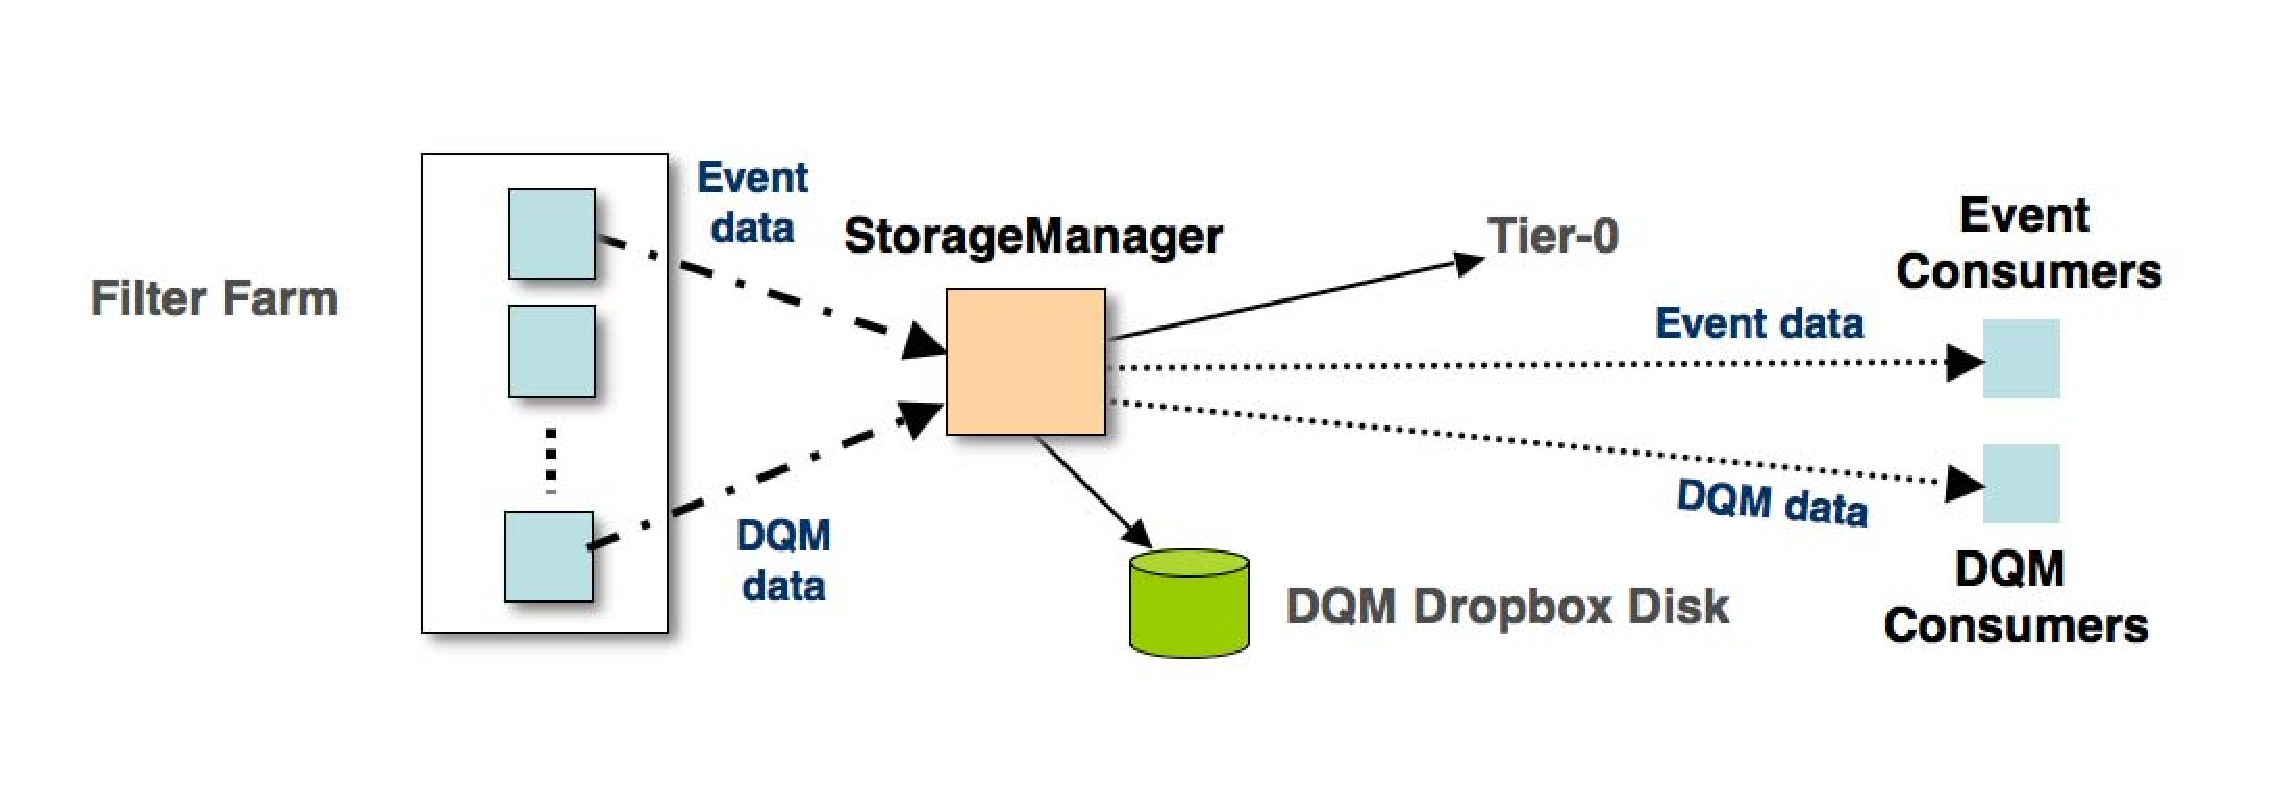
\includegraphics[width=5.5in]{Software/schematic_simple}
    \caption{Functional schematic.}
    \label{fig:schematic_simple}
  \end{center}
\end{figure}

\subsubsection{Software Responsibilities}

The Storage Manager project software task has well defined  responsibilities. The
functions of the code needed are listed below. 

\begin{itemize}
\item Serialize data into a byte stream for network transfer.
\item Create and maintain the serialized data format.
\item Provide input modules to deserialize and reform the data for the framework.
\item Receive data from all HLT processes in the Filter Farm.
\item Output event data in streams based on trigger bits.
\item Communicate and interact with Tier-0 for data transmission to Tier-0.
\item Serve event data and DQM data to consumers.
\item Receive DQM data, sum histograms and output to DQM Disks.
\end{itemize}

Much of the Storage Manager software is well integrated within the standard
CMS offline framework. In fact the base classes for the serialized data input
source and serialized data output modules are provided and maintained by the
CMS framework group.

\subsubsection{Requirements and Dependencies}

The Storage Manager runs in the CMS online system which is implemented within
the XDAQ framework. The Storage Manager application must be a XDAQ application
operating within the CMS DAQ and configured, controlled, and monitored by the
CMS Run Control.

The Storage Manager must be able to handle the required data rates and the
primary event data collection and output must not be compromised by the other
functions of the Storage Manager.

The event data and DQM data consumers must be able to receive the data using a
standard CMS EDM offline framework job, or a CMS XDAQ consumer application.
There is currently no requirement for remote consumers, {\em i.e.} ones that operate
from outside of the experimental private network.

The strategy of the Storage Manager group is to reuse as much of the code in
the CMS offline framework, the CMS DAQ, and the DQM framework. This
integration means that the SM code is highly dependent on these three 
subsystems.

\flushleft{\em Handling of Events with Different Data Products}

The HLT process will produce data where events can have different data products. An example
use case is the production of the following streams:

\begin{itemize}
\item Physics stream saving all main products (data branches)
\item Calibration stream saving only a few data products; high rate
\item Debug physics stream saving all main products and in addition many intermediate 
data products for debugging; low rate
\item Exception stream where HLT modules have failed; very low rate
\item Auto-accept (small fraction of all events passing L1); low rate
\end{itemize}

Separately there is an Error Stream that does not actually go through the HLT. This 
Error stream is for events that cause a HLT process to die or time out. These events 
go directly from the Resource Broker to the Storage Manager.

Due to a limitation of the offline software framework, all events in a particular output
stream file must have exactly the same set of data products. Events with different
data products cannot be mixed into the same file.


\subsection{Architecture}

The approximately 640 Filter Farm nodes will be split into 8~(or multiple of 8) separate
slices or subfarms. Each subfarm will have its own Storage Manager application
instance as illustrated in Fig.~\ref{fig:SM_architecture_base}. A separate XDAQ 
SM Proxy Server application collects events at a low rate from the
Storage Managers of each subfarm to serve to event consumers. The SM Proxy
Server application also collects DQM data and sums the DQM histograms before
outputing these summed DQM data to the DQM disks. All Storage Manager
instances and the  SM Proxy Server
application sits inside the CMS DAQ private network.

Each Storage Manager application also has event data and DQM data server
functions, however in normal running the Storage Managers will be isolated from
all consumers by the SM Proxy Server.

\begin{figure}[hbtp]
  \begin{center}
    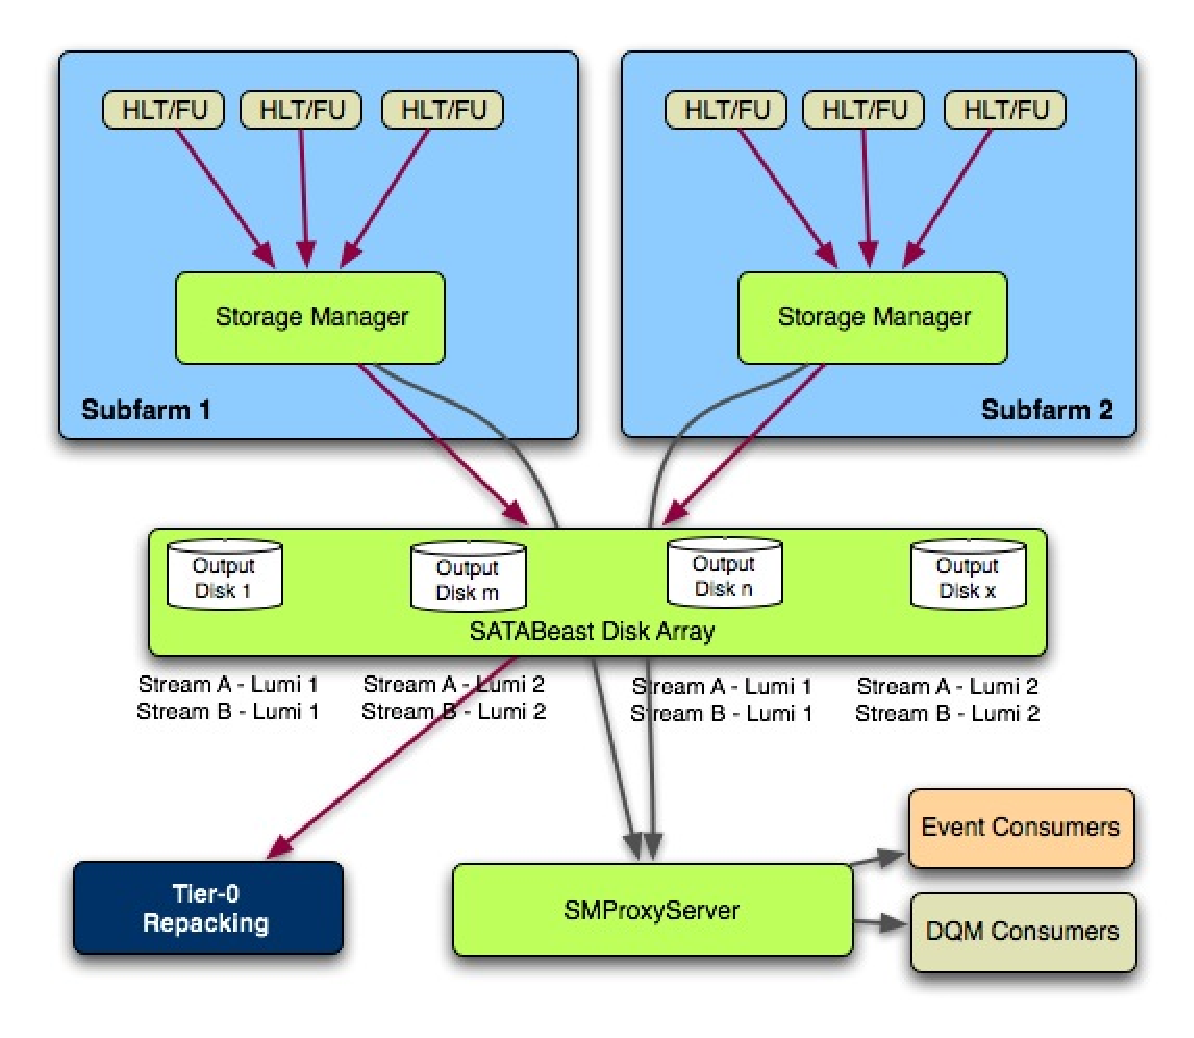
\includegraphics[width=4.5in]{Software/SM_architecture_base}
    \caption{Architecture with subfarms.}
    \label{fig:SM_architecture_base}
  \end{center}
\end{figure}

\subsubsection{Routing of Events in the Storage Manager}

It was decided to implement multiple output streams with different data products by using
multiple HLT output modules, where each output module gives events with a certain
data product selection.
The HLT output module, Resource Broker, and Storage Manager software need to handle 
the following issues:

\begin{itemize}
\item HLT output modules are able to drop products independently (no assumption 
that one output module will contain the whole superset of data products).
\item An event can satisfy the selection for multiple output modules, and thus need 
to go to multiple streams in the Storage Manager with the correct data products.
\item The Storage Manager must write streamer files that are readable and can be 
converted to Root files irrespective of what data products are kept for the stream (file).
\end{itemize}

The data for each HLT output module is tagged with the output module identifier,
 the SM uses this output module id as well as the event trigger bits to direct events to the
 correct output stream file. The HLT and SM configuration are thus coupled and must be 
 correctly setup to route events to the correct output streams.


\subsection{Software Components}

In this section we describe each of the software components that form the
Storage Manager software project. These are represented by the circles/ovals in
Fig.~\ref{fig:schematic_wproxy}. The hardware view from 
Fig.~\ref{fig:system} is used in Fig.~\ref{fig:sm_hardware_wsoftware}
to illustrate where the software components run.

\begin{figure}[hbtp]
  \begin{center}
    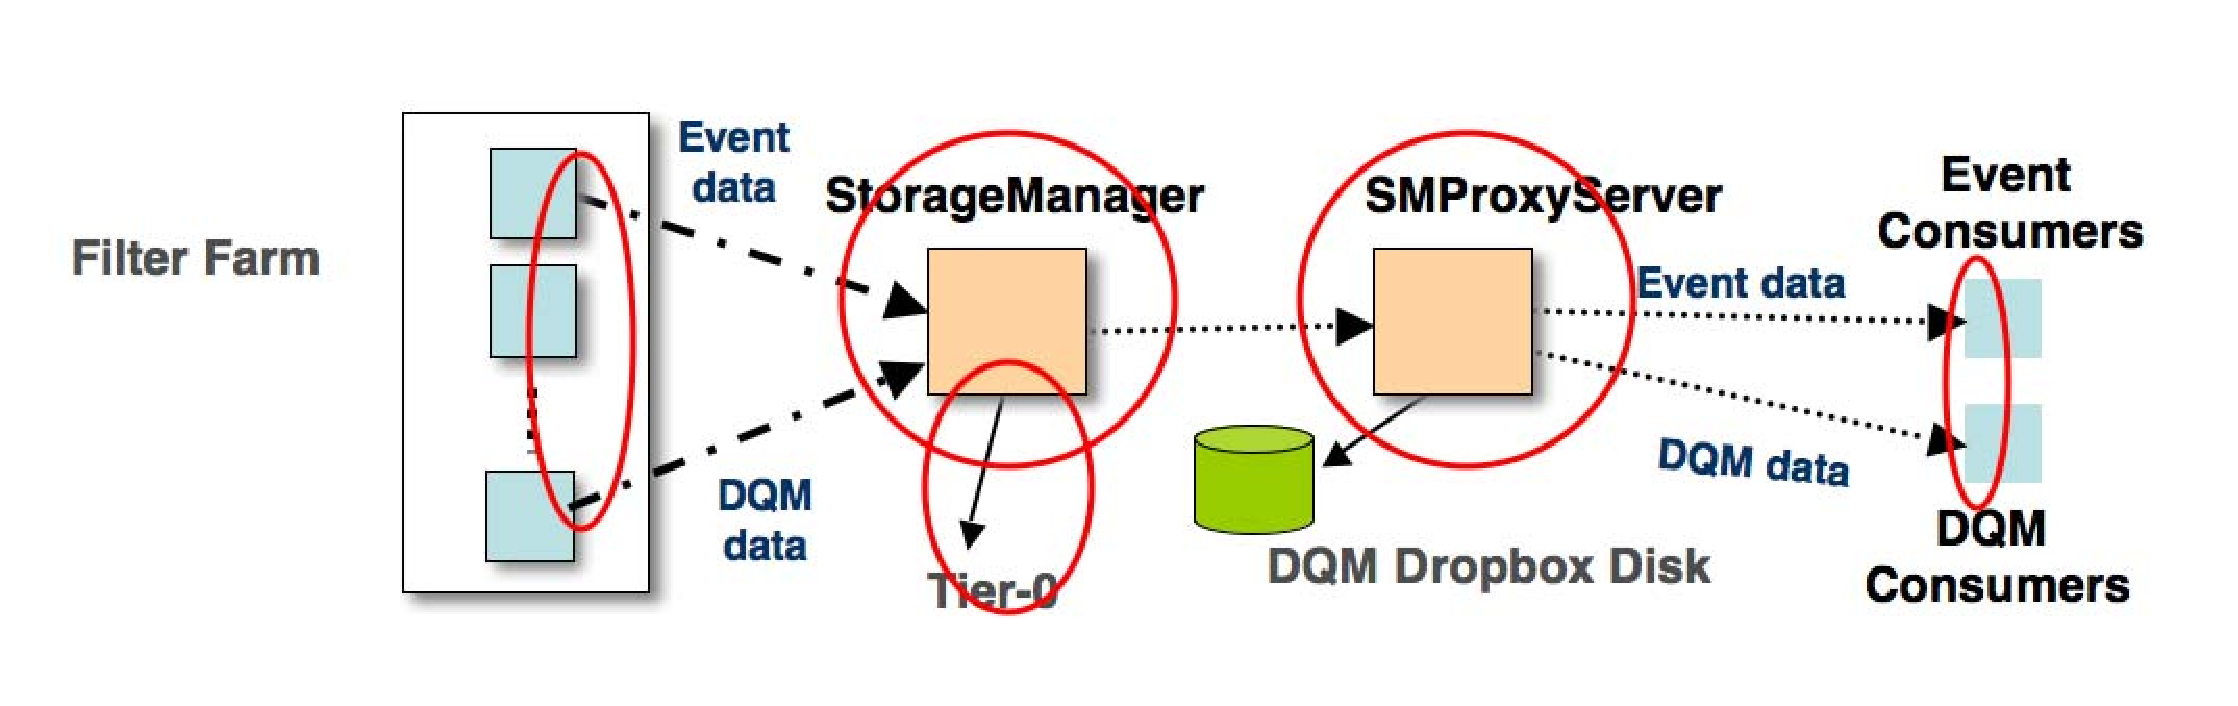
\includegraphics[width=5.5in]{Software/schematic_wproxy}
    \caption{Functional schematic with subfarms.}
    \label{fig:schematic_wproxy}
  \end{center}
\end{figure}

\begin{figure}[hbtp]
  \begin{center}
    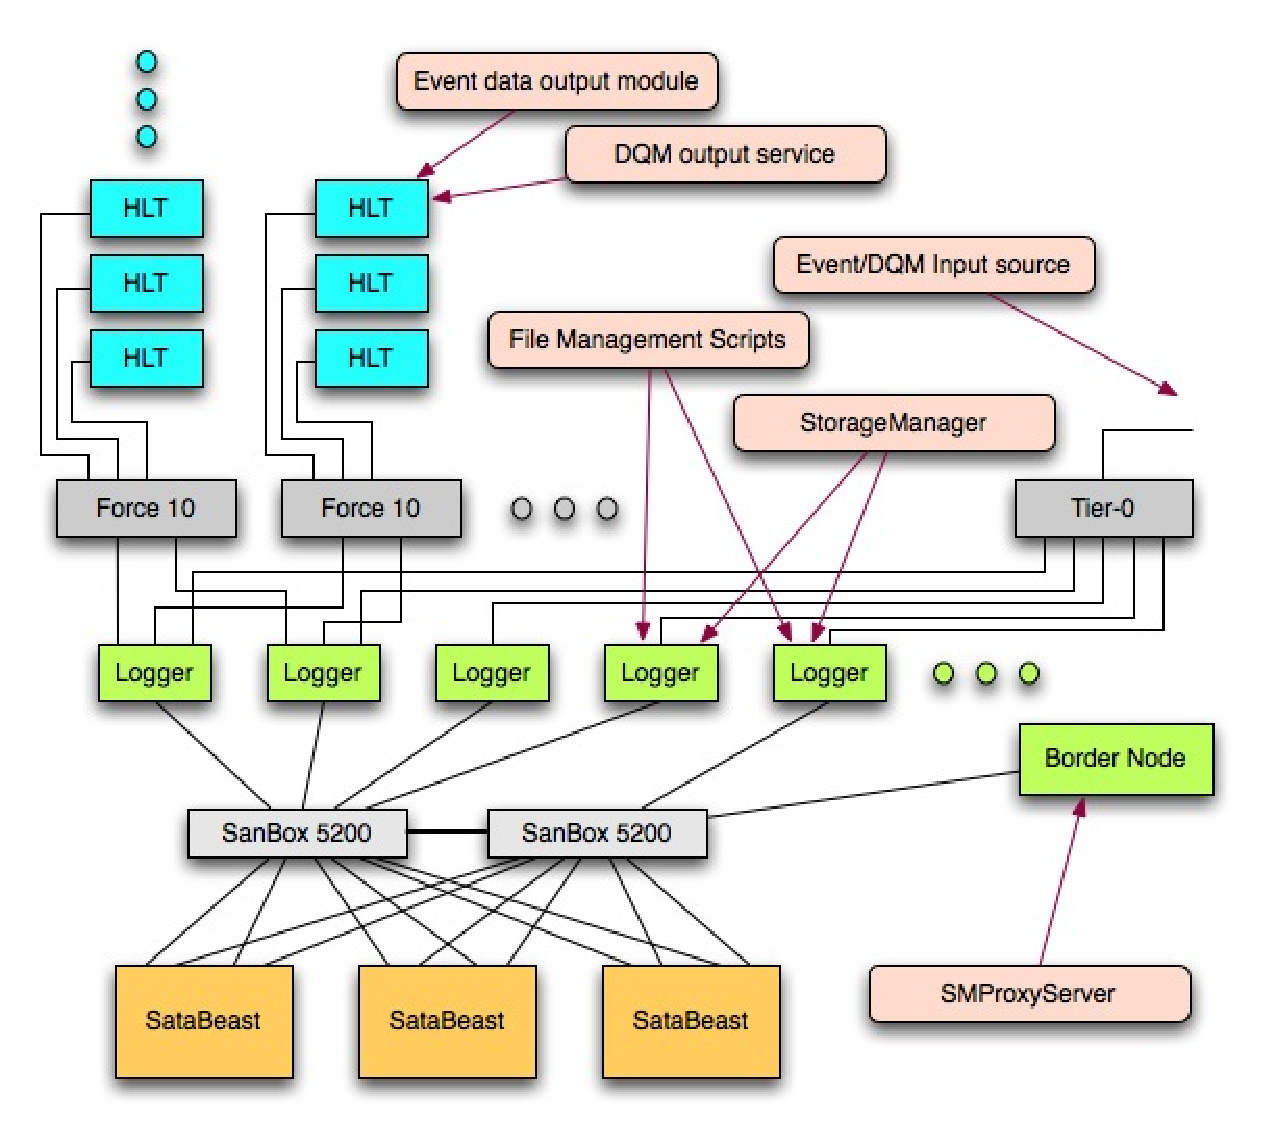
\includegraphics[width=4.5in]{Software/sm_hardware}
    \caption{Hardware view showing where the software components run.}
    \label{fig:sm_hardware_wsoftware}
  \end{center}
\end{figure}

\subsubsection{Output and Input Modules}

The Storage Manager group provides the CMSSW framework (FW) 
output module for the HLT process. In
the output module the event data are serialized into a ``blob'' of bytes for
transfer over the network to the Storage Manager. The actual transfer is
done by the Resource Broker running the on the HLT Filter Farm node via
the I2O facility in XDAQ. This is illustrated in Fig.~\ref{fig:ps_fudesign}.
The ``data blob'' is written to shared memory which is managed by the
resource broker.

\begin{figure}[hbtp]
  \begin{center}
    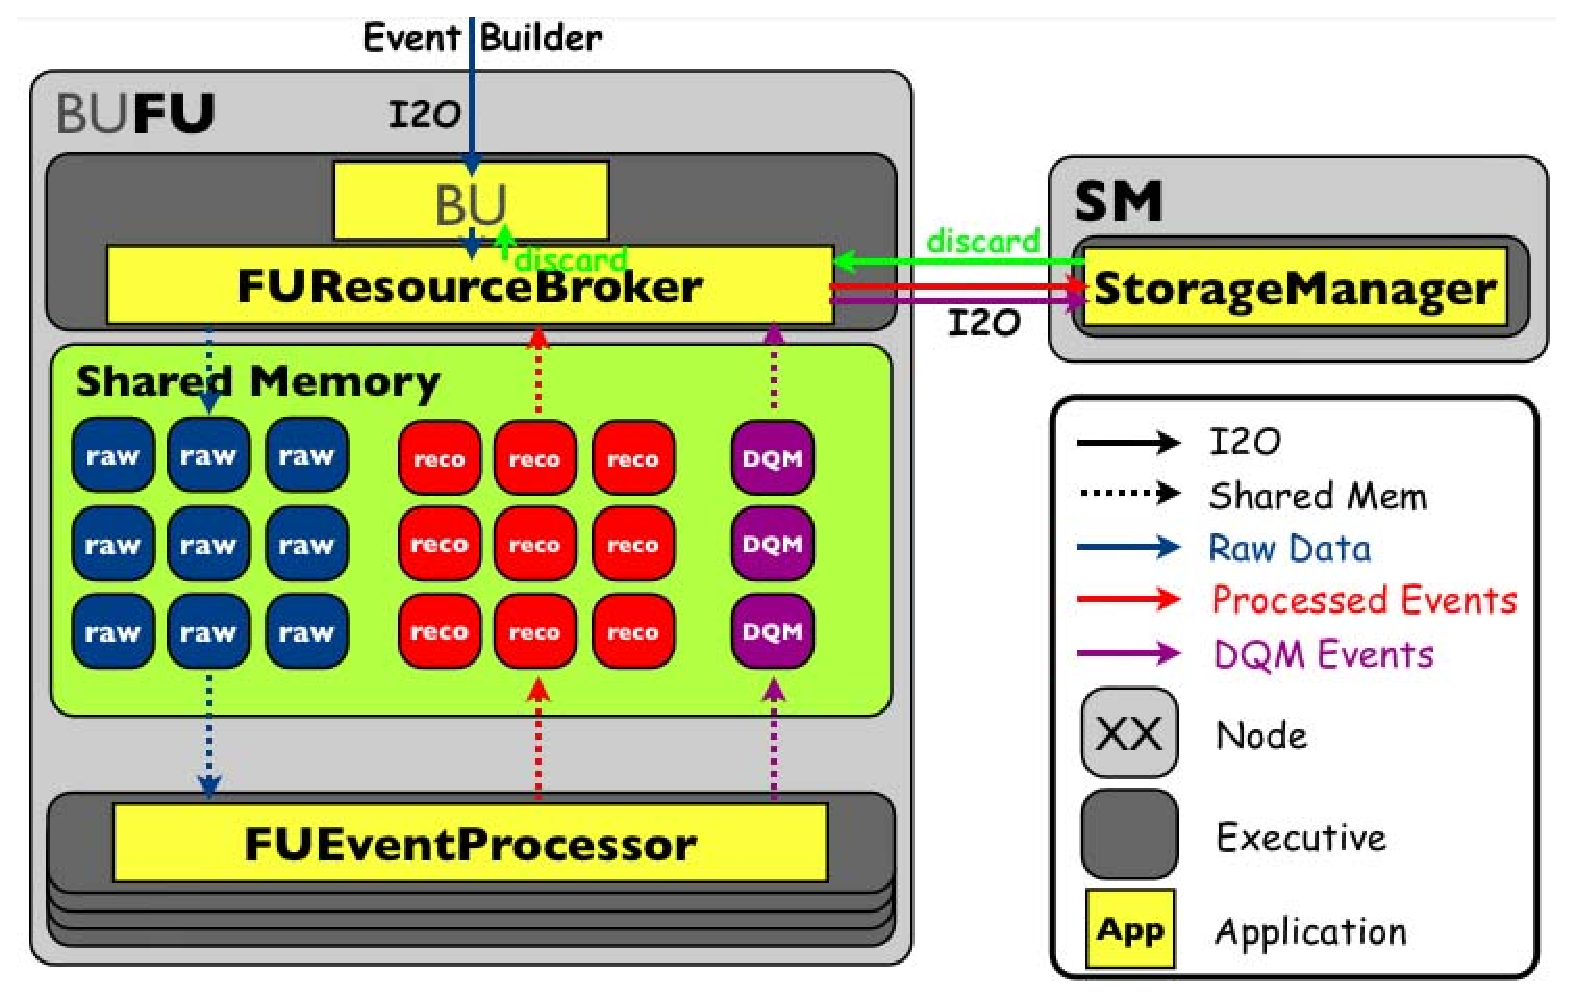
\includegraphics[width=5.5in]{Software/ps_fudesign}
    \caption{Schematic showing the mechanism for data transfer between the
HLT process (FUEventProcessor) and the Storage Manager.}
    \label{fig:ps_fudesign}
  \end{center}
\end{figure}

Since the maximum size of I2O frames is 256~KB, and the actual I2O frame
size used in the CMS online is smaller (64~KB), the resource broker 
splits the data for each event into as many fragments as needed, wraps each fragment with
appropriate I2O headers and sends them to the Storage Manager. The code for
doing the split of the ``data blob'' was initially provided by the Storage Manager
group though it now resides in the Resource Broker software package and
maintained by the CMS DAQ group.

The output module is a plugin module of the CMS offline framework and can be
used in either a standard CMS offline job (using cmsRun), or within the online
HLT process. The online HLT process uses an instance of CMS offline framework
event processor running in an asynchronous mode, and basically has the same
features as an offline event processor except its execution can be controlled
by the CMS Run Control.

The output module inherits from an output module class provided by the CMS
offline framework group, thus the main maintenance load is with the data
serialization. The output module is actually a templated class and another
output module using the same template is also maintained that writes out
streamer files instead of to shared memory. This additional streamer file
output module is used internally for testing purposes.

The Storage Manager group provides a DQM output service plugin module.
The output service uses the standard offline framework hooks for its
processing schedule, and the main function is to serialize the
DQM data and write to shared memory.

The Storage Manager group also provides two input source plugin modules,
one for streamer file input and one for network input. Both inherit from
a base input source provided and maintained by the CMS framework group.
The streamer file input source is used primarily by the Tier-0 group
but is also used internally for testing purposes. The network streamer input
module is used for event data consumers for online monitoring.
These input sources do the deserialization needed to convert the serialized
data back into CMS framework event objects.

The network input source used by the online consumers use cURL to
interact with the HTTP server of the Storage Manager application, and uses a 
HTTP GET command to receive data in a binary stream.

These input sources are not used inside the Storage Manager itself.
No deserialization of the event data is done in the Storage Manager, and it does not
use the CMS framework event processor. 
Deserialization of DQM histogram data may take place in the Storage Manager
so that the same histogram from multiple HLT processes can be summed before
sending to the SM Proxy Server.
Details of the Storage Manager and SM Proxy Server input
and processing is given below in the respective application description sections.

\subsubsection{Serialization and Deserialization}

A serialized data format was created for the serialized data. Originally this
format was to be a completely temporary format used only for the network
transfer of event data to the Storage Manager. The Storage Manager would then
write out standard CMS ROOT files. During the testing of the first prototype
of the Storage Manager we found that the deserialization performance was too
poor to write out standard CMS ROOT files. Instead in the second prototype
we wrote out flat binary files, called streamer data files, these are basically
the concatenation of each of the event serialized data messages
sent over the network.

\begin{figure}[hbtp]
  \begin{center}
    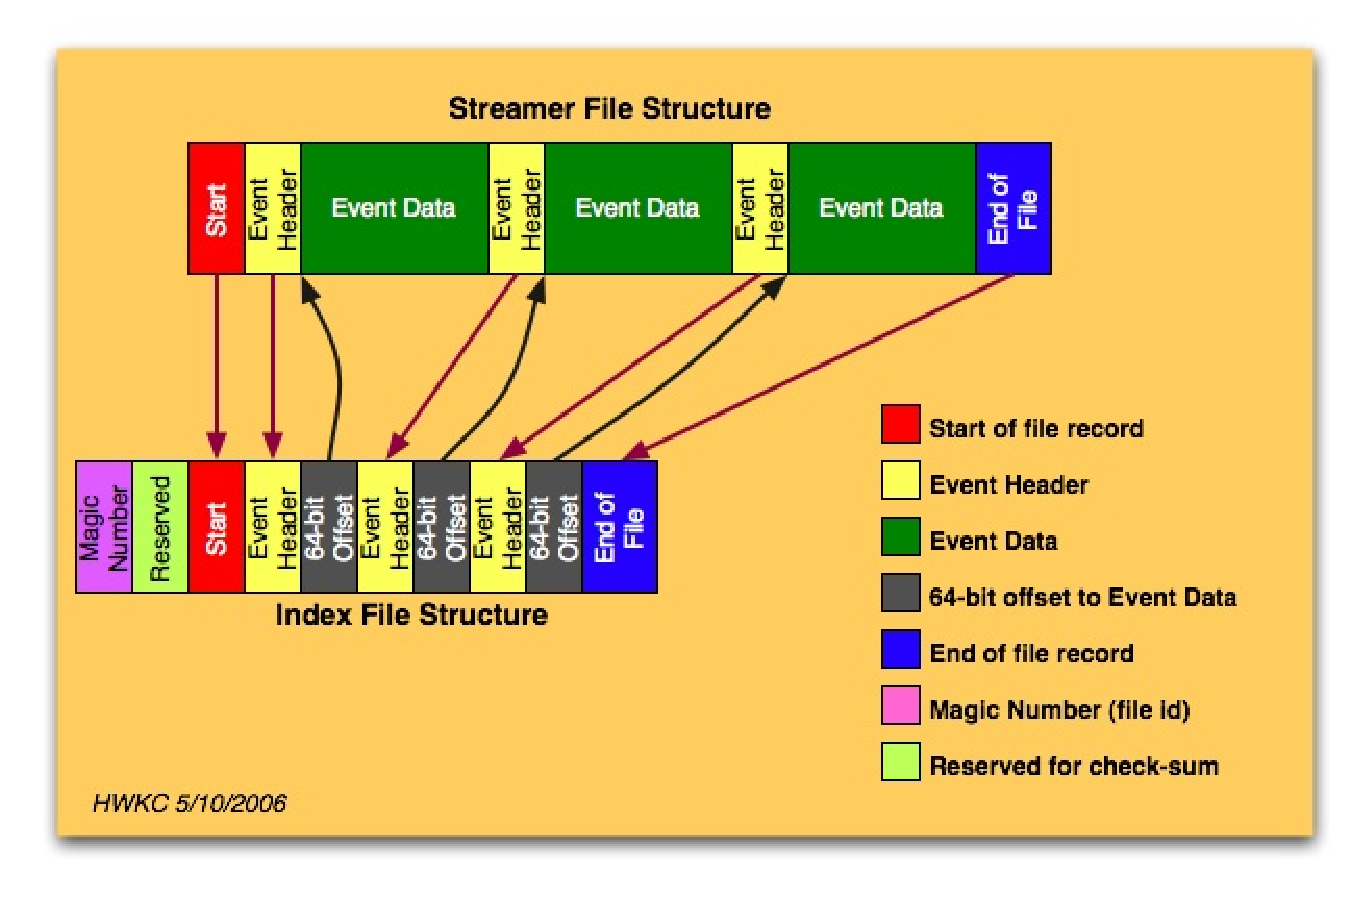
\includegraphics[width=5.5in]{Software/sm_messages1}
    \caption{Schematic showing the format of Streamer files and index files.}
    \label{fig:sm_messages1}
  \end{center}
\end{figure}

The streamer file format is illustrated in Fig.~\ref{fig:sm_messages1}. The file
consists of a start of file record, and an event record for each event, and
an end of file record is placed at the end of the streamer file. The event
record consists of an event header and the event data.

The actual formats of the start of file record, the event header and data, and the
end of file record are given schematically in Fig.~\ref{fig:sm_mess_structure}.
The formats of the start of file record, and the event record are exactly the
same as the format of messages used to transfer data from the HLT process to the
Storage Manager. This has the advantage of having less code for the Storage
Manger group to maintain.

\begin{figure}[hbtp]
  \begin{center}
    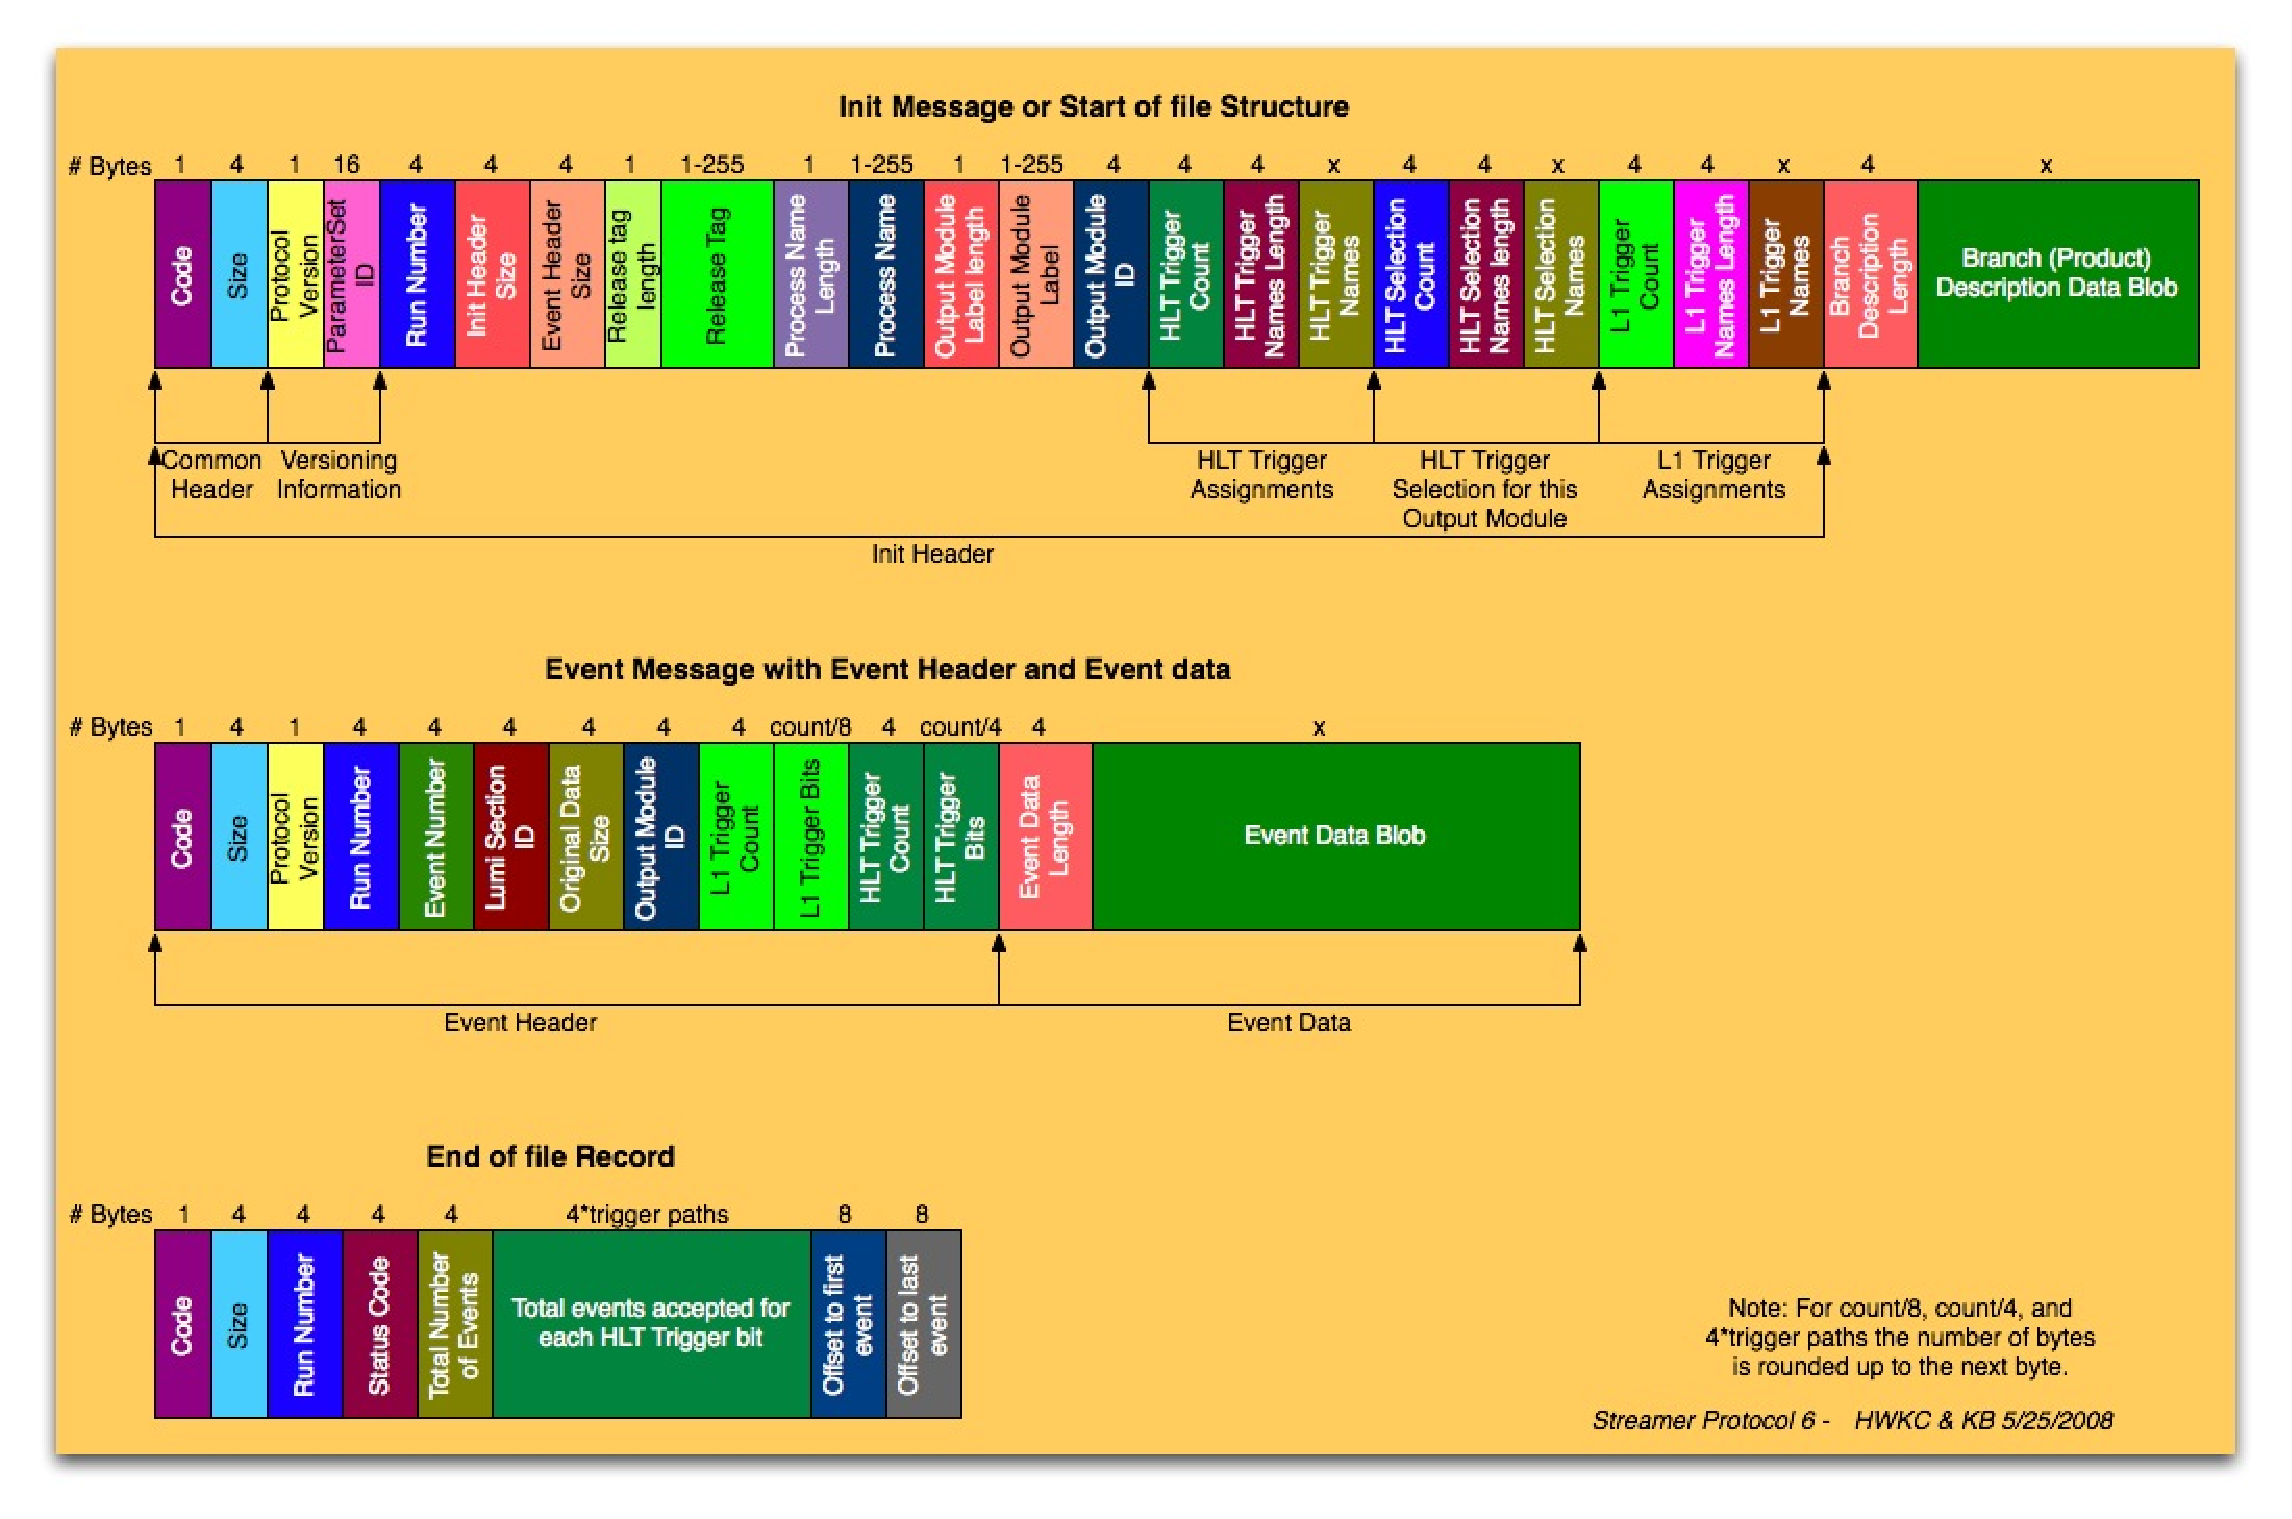
\includegraphics[width=6.0in]{Software/sm_mess_structure}
    \caption{Schematic showing the format of serialized data messages.}
    \label{fig:sm_mess_structure}
  \end{center}
\end{figure}

At the start of a run, each HLT process output module
sends an INIT message to the Storage Manager.
This INIT message is the same as the start of file record. For each run, the data 
for the first received INIT message of each output module
are saved for output as the start of file 
record for the streamer files. The data for each event is transmitted by the
HLT processes to the Storage Manager in the form of an event message which is
the same as the event record. It consists of the event header and the event
data. The event data is just the serialized ``data blob'' mentioned above
preceded by its size in bytes.

Besides the streamer files, the Storage Manager also writes out one index file
per streamer file. The format of these index files are given in Fig.~\ref{fig:sm_messages1}.
The index file contains the same start of file and end of file records as the streamer
file, however for each event it contains only the event header and the byte offset
for that event's data in the corresponding streamer file. The index file is intended
for use during Tier-0 processing to aid in random access reads of streamer files, and
is thus only temporary. The index file has the same name as the streamer file but with
an extension of ``.ind'' instead of ``.dat''. At this time, the Tier-0 group have yet to decide
if these index files will be used.

\begin{figure}[hbtp]
  \begin{center}
    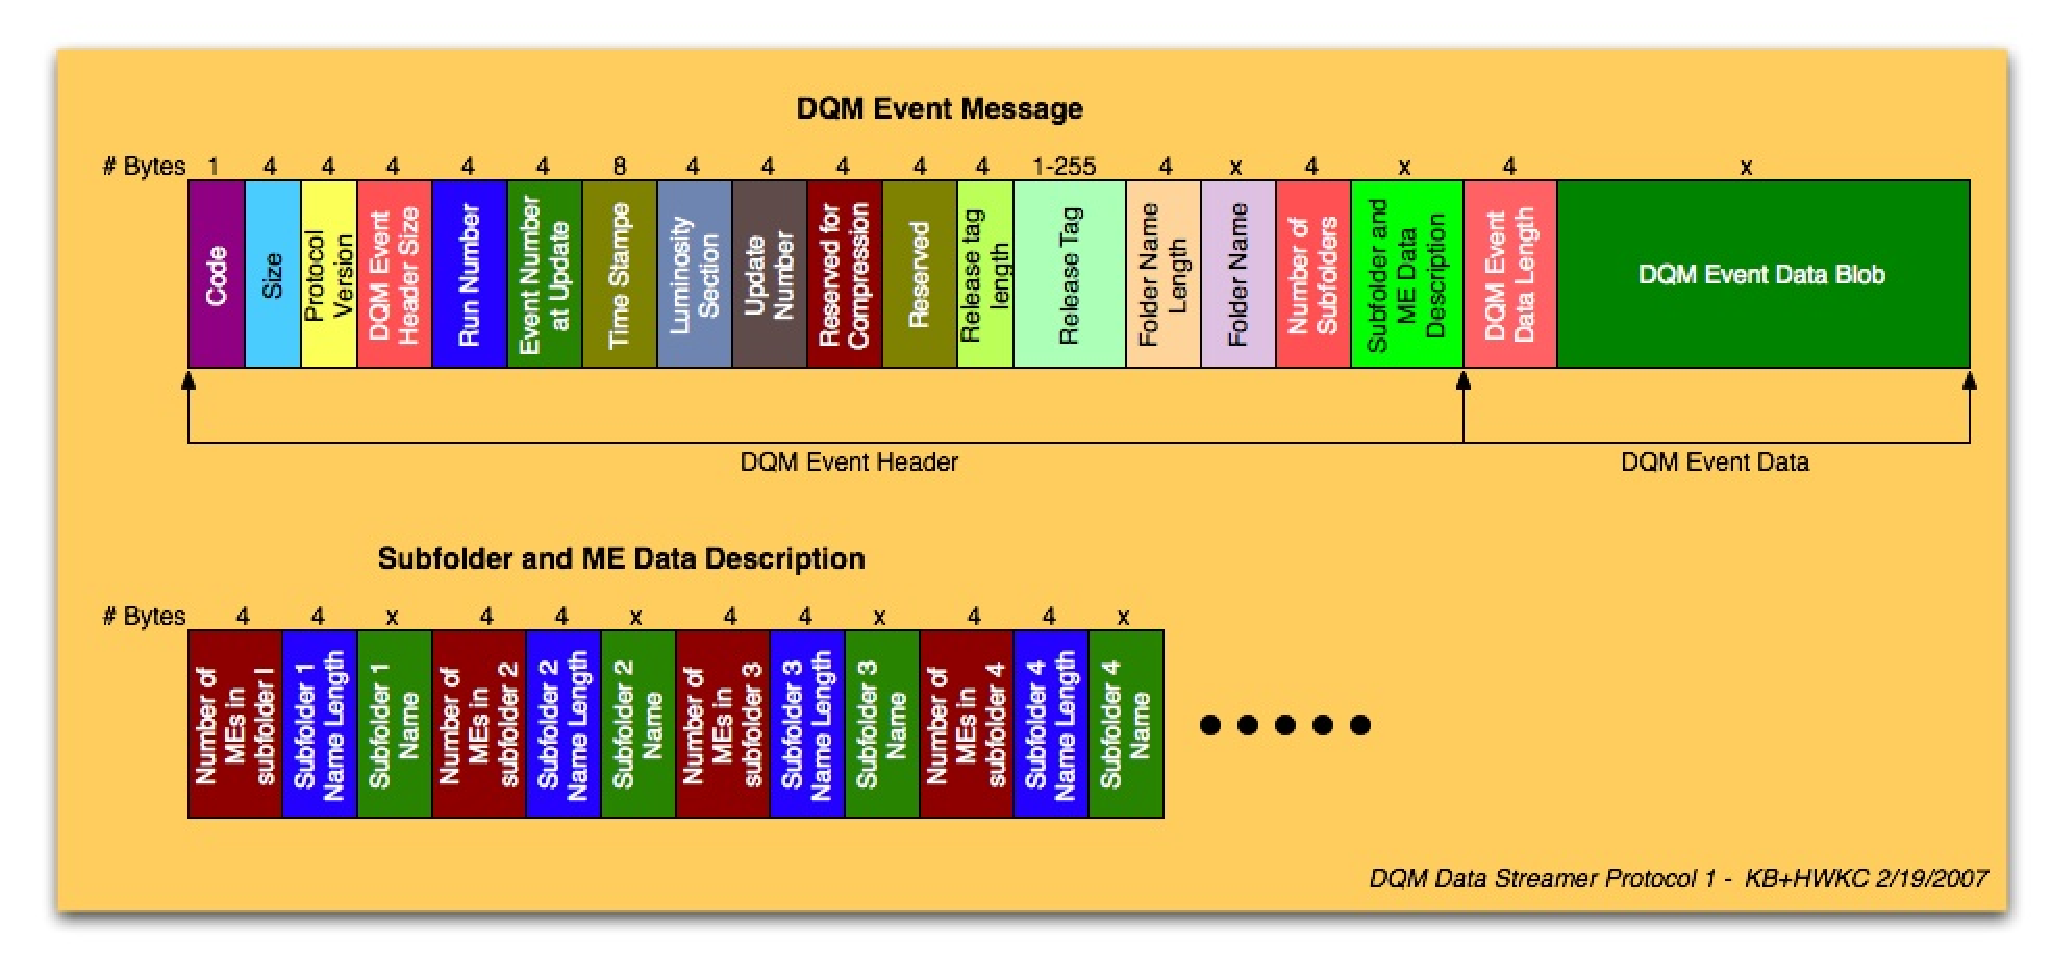
\includegraphics[width=6.0in]{Software/sm_dqmmess_structure}
    \caption{Schematic showing the format of serialized DQM messages.}
    \label{fig:sm_dqmmess_structure}
  \end{center}
\end{figure}

The transmission of DQM data from the HLT processes to the Storage Manager is done
using serialized DQM data messages. The format of these messages are given in
Fig.~\ref{fig:sm_dqmmess_structure}. The DQM data are essentially ROOT
histograms, and integers, floats, and std::strings stored as TObjects. These
data are organized into a number of (top-level) folders and subfolders. 

The DQM data for each top-level folder is serialized into a ``blob'' of bytes and
placed in its own DQM data message, and preceded by some header information as
shown in Fig.~\ref{fig:sm_dqmmess_structure}. The DQM data are sent at each
``update interval''. Usually this update interval is at the end of a luminosity
section (nominally 93~seconds).

Both the serialization of event data and the DQM data is done using ROOT.
The event data in the CMS framework is stored using ROOT TTrees, and
the serialization is done using the class descriptions of the event data
objects in ROOT for the particular version of the offline CMSSW version used. 
Only a subset of the event meta data is written out to the streamer file. 
%Normally it is assumed that the streamer file is the first step in the data chain, where
%the first process is the HLT process. Note that the HLT+SM is identified as
%a single process. This assumption has implications in the playback of real
% or MC data files in the online for testing purposes.
The chosen meta data are put into a data structure for which ROOT can generate
an automatic class description.

The start of file record in each streamer file includes the version of CMSSW used
and the ``branch descriptions''. These branch descriptions
 include the identifier of each of the event
data branches. However the class descriptions themselves are not stored in
the start of file record. To deserialize the data back to the original data objects
we load the class descriptions for each of the data branches using the 
appropriate CMSSW libraries. To be safe this means that the version of CMSSW
used to deserialize the streamer file should be the same as that used for
writing that streamer file. 

There is no provision for schema evolution for the
streamer files since they are temporary data formats. However this has implications
for the online event data consumers.

The DQM data contain
only histograms and simple types and std::strings, no special class descriptions
are needed to deserialize these data.


\subsubsection{Storage Manager Application}

The functions of the Storage Manager XDAQ application are listed below.

\begin{itemize}
\item Receive event data and DQM data in the form of I2O frames and
reform the fragments.
\item Output event data streamer files based on the per run configuration 
and the per event trigger bits.
\item Communicate with Tier-0 for the transfer of streamer files to Tier-0.
\item Take online consumer registrations and serve event data and DQM
data to registered online consumers.
\end{itemize}

After the experience with the first prototype of the Storage Manager it was
decided that no (real) processing is done in the Storage Manager application
since even the deserialization was found to be too CPU intensive for the
Storage Manager to keep up with the design incoming data rate.

\begin{figure}[hbtp]
  \begin{center}
    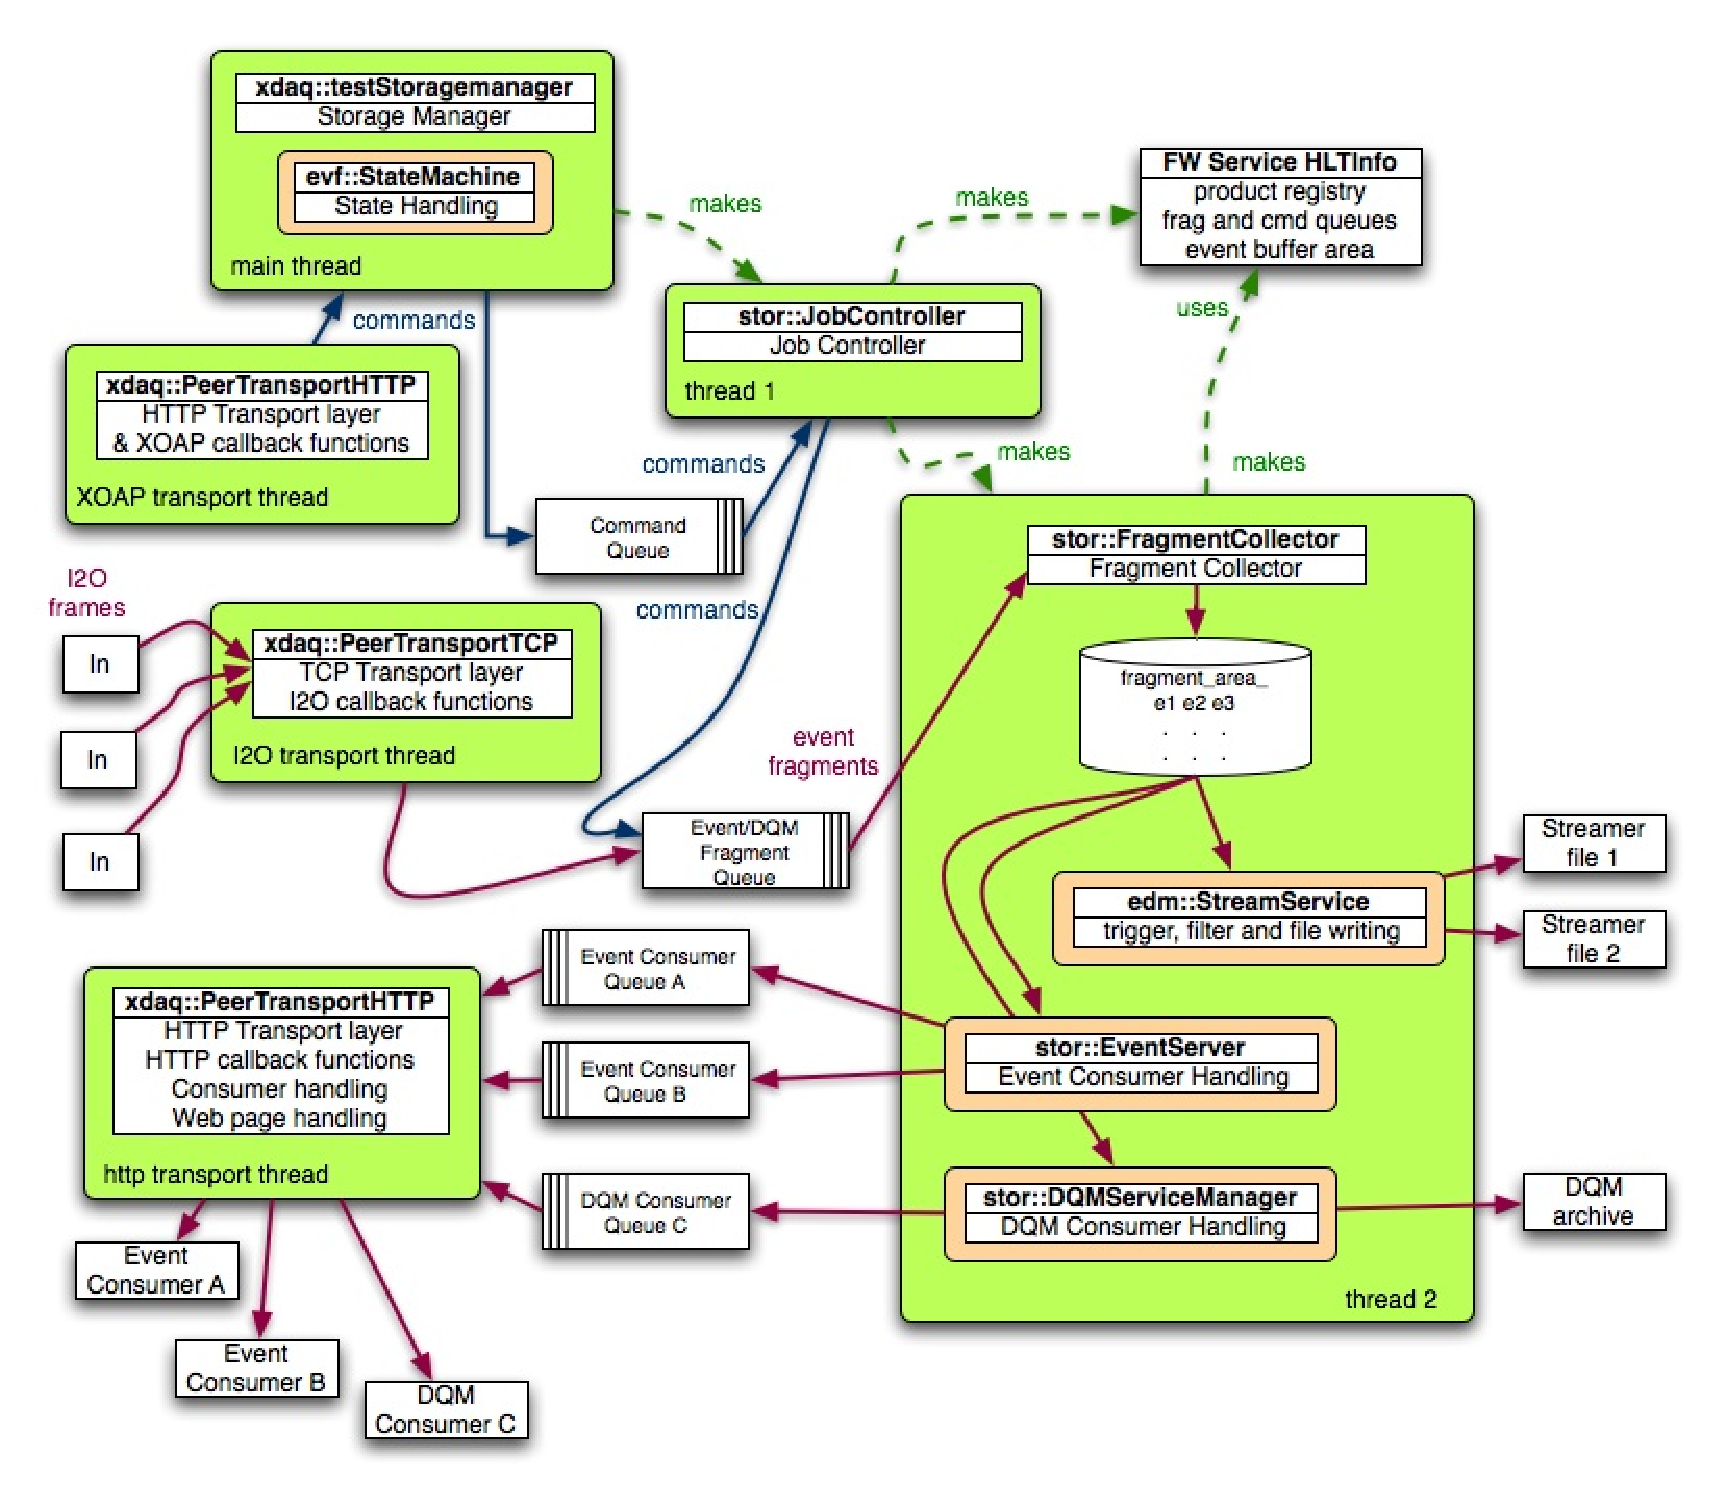
\includegraphics[width=6.0in]{Software/SM_System}
    \caption{Design of the Storage Manager application.}
    \label{fig:SM_System}
  \end{center}
\end{figure}

Figure \ref{fig:SM_System} illustrates the design of the Storage Manager
application. The StorageManager XDAQ application runs within the xdaq.exe
executable in the main thread,
but basically all the processing is done in other threads of this application.
There are three transport callback threads, one for I2O, one for XOAP, and one
for HTTP.  Additionally there are two other threads started from the
StorageManager application itself, the JobController thread, and the
FragmentCollector thread. The functions of these processing threads are
given below.

\begin{itemize}
\item {\em XOAP transport thread.} Commands to the Storage Manager are sent
via XOAP (XML) messages, and various XOAP callback functions are defined in
the Storage Manager application to handle these commands. These commands
include commands to configure, start, pause, and end (halt)  the
Storage Manager application.

\item {\em I2O transport thread.} The incoming event data and DQM data I2O frames
trigger I2O callback functions that run in the I2O transport thread. The I2O callback
functions are defined in the Storage Manager application and essentially just place 
the appropriate data fragments with identifiers into
the event/DQM fragment queue. If the SM instance is run on a PC with multiple
network interface cards (NICs), there can be one I2O transport thread per NIC.
The event/DQM fragment queue is protected by a mutex.

\item {\em HTTP transport thread.} HTTP callback functions are also defined in
the Storage Manager application and handle various tasks. The tasks include
generating web pages with various monitoring data about the Storage Manager,
called application web pages and these are the most direct means of monitoring
each XDAQ application besides looking at that application text console. Other
HTTP callback functions handle online consumer registration and sending data
to the online consumers.

\item{\em JobController thread.} The JobController creates shared data structures like
the fragment queue and creates and starts the FragmentCollector thread. The Storage
Manager can issue commands to the JobController thread by placing them in the
command queue. In the running state the JobController thread just reads the
command queue and reacts to what is read. The command queue is a blocking queue
so that if empty a read will block until something is placed in the command queue. The 
command queue is protected by a mutex.

The JobController thread can control the FragmentCollector thread by placing
commands in the (event/DQM) fragment queue. The fragment queue is a blocking
queue like the command queue and also protected by a mutex.

\item{\em FragmentCollector thread.}  In running mode the FragmentCollector thread
reads the fragment queue and processes event fragments, DQM data fragments,
and also commands like an end of run or a halt. The data fragments are collected and
reformed into the serialized event data or DQM data. 

Once reformed the serialized data for an event is written out to streamer files based
on the trigger bits for the event and the initial per run configuration of the Storage Manager.
The output files can be written out in streams, for example a physics stream, a
calibration/alignment stream, and a debug stream. In each SM instance,
the data for each luminosity section
for each stream is written to one file. The data for the event is also passed to the
event server which determines if it needs to be placed in any online consumer queues.

Reformed DQM data are passed to the DQMServiceManager which can be configured to sum up
histograms for the same update. Once the histograms are summed they are written out to
the DQM disks. These DQM data are also passed to the
DQMEventServer which determines if it needs to be placed in any DQM consumer queues.
\end{itemize}

The state of the StorageManager application is kept in a Finite State Machine. This
is implemented using FSM code provided and maintained by the Event Filter Group
which is part of the CMS DAQ group. This provides a uniform set of states and
allowed transitions for XDAQ applications within the Event Filter Group. The
state chart for the StorageManager application is illustrated in Fig.~\ref{fig:sm_fsm_chart}.

\begin{figure}[hbtp]
  \begin{center}
    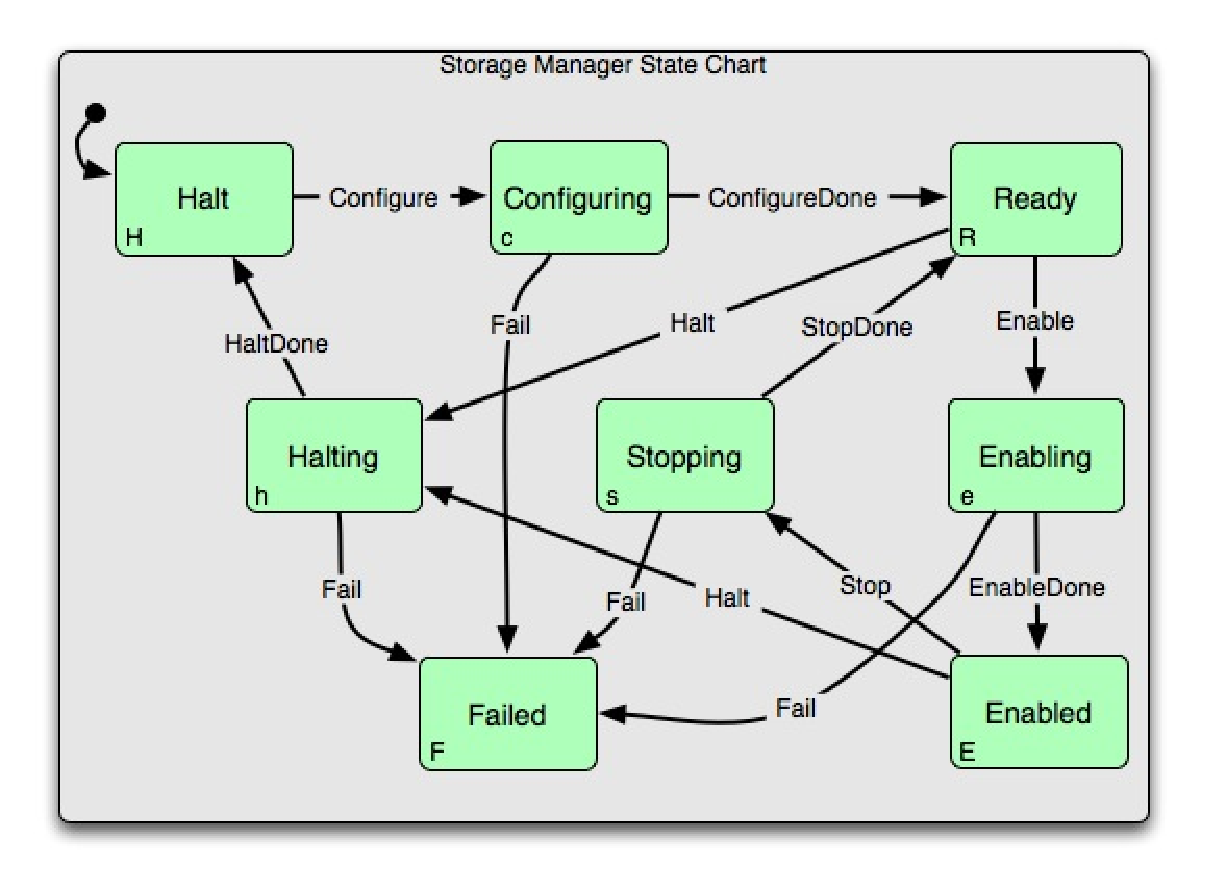
\includegraphics[width=4.5in]{Software/sm_fsm_chart}
    \caption{Storage Manager State Chart}
    \label{fig:sm_fsm_chart}
  \end{center}
\end{figure}

The online event and DQM consumers interact with the Storage Manager event and
DQM servers through HTTP GET and POST commands, and data are transferred using
a binary stream. Online consumers register with the Storage Manager and get
data via a pull mechanism, polling at a maximum rate of a several Hz. The
event and DQM servers limit the data rate and bandwidth to online consumers to
ensure that the primary function of the Storage Manager is not compromised.

Copies of the data are minimized in the Storage Manager during its execution
loop. The received data fragments remain in the XDAQ memory pool
until all fragments are received. At this point the data are copied and
concatenated together to reform the serialized ``data blob" before being
written out to streamer files. The memory for this event data in the
XDAQ memory pool is
then released, but the event server retains a
copy of this event data. Pointers to this single copy of the data
are used in the consumer queues.


\subsubsection{Storage Manager Proxy Server Application}

With multiple StorageManager instances, one for each subfarm, online
consumers must be able to get events from multiple Storage Managers. This is
one of the functions of the SMProxyServer XDAQ application. The design of the
SMProxyServer is illustrated in Fig.~\ref{fig:SMProxyServer_System}.

\begin{figure}[hbtp]
  \begin{center}
    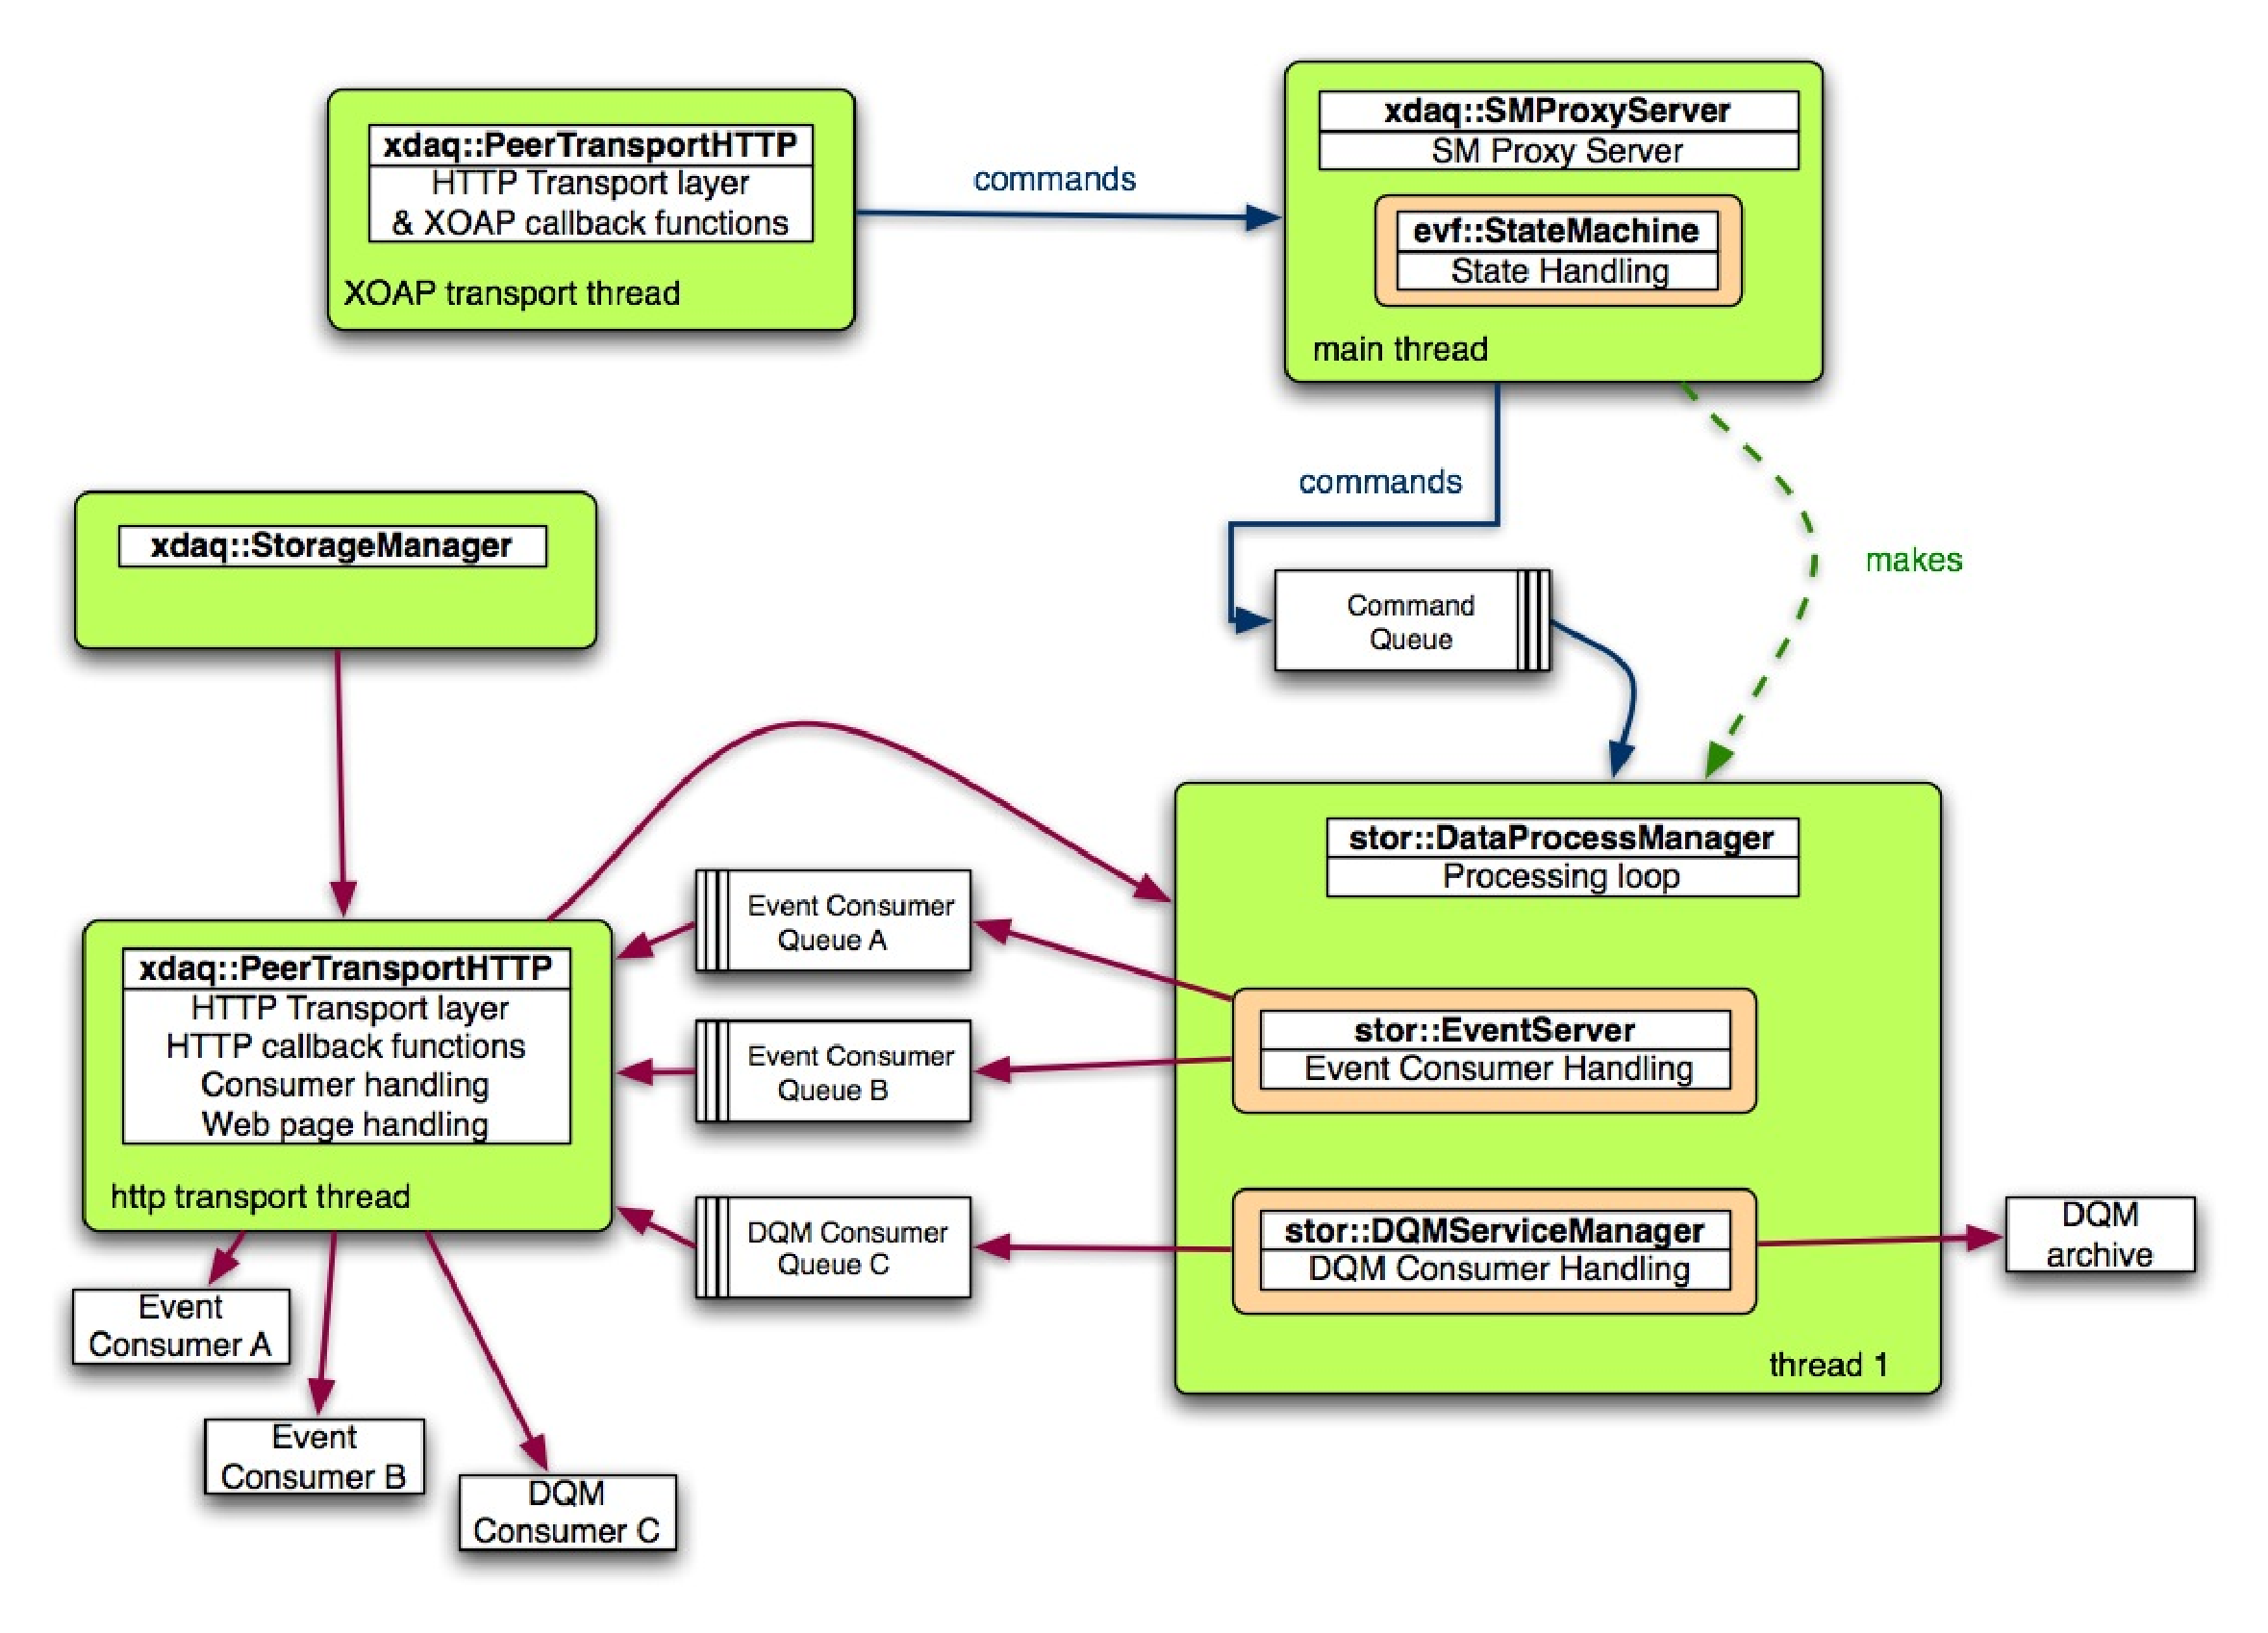
\includegraphics[width=5.5in]{Software/SMProxyServer_System}
    \caption{Design of the Storage Manager Proxy Server application.}
    \label{fig:SMProxyServer_System}
  \end{center}
\end{figure}

The SMProxyServer gets event data and DQM data from each of the StorageManagers
like an online consumer. The SMProxyServer also
registers itself with each of the StorageManager applications. However unlike
a regular online consumer, the SMProxyServer can receive data from
multiple HLT output modules.  The event server in each SM instance can
limit the rate of the data to the SM Proxy Server.

As much of the StorageManager code as possible is used in the
SMProxyServer to reduce the amount of code that needs to be maintained.
Instead of the JobController thread and the FragmentCollector thread the
SMProxyServer only has a DataProcessManager thread. This DataProcessManager
thread manages the registration of the SMProxyServer with all StorageManager
instances, and processes commands in the command queue.

The SMProxyServer functions as an event and DQM server to serve online consumers.
In normal running the online consumers would actually only connect to the
SMProxyServer application. This isolates the StorageManager applications from
the online consumers.

Finally the SMProxyServer receives DQM data from each of the StorageManager
applications and sums up the histograms from each StorageManager instance
for the same update and saves them to the DQM disk.

The SMProxyServer application uses the same state machine code as the 
StorageManager application and the state chart is the same as that given
in Fig.~\ref{fig:sm_fsm_chart}.


\subsection{\label{sec:fpt0}File Processing, and Communication and interaction with Tier-0}

For each stream and each StorageManager instance one output file is written
per luminosity section. Each SM instance uses volumes on separate disk arrays 
(see the hardware section, Section~\ref{sec:stohard}).

Events arrive asynchronously to the Storage Manager depending on the processing
time for each event in the HLT process. On the arrival of an event from a
new luminosity section a new streamer file is created for this luminosity section,
and an entry is created in the online database for this file. 
The arrival of an event from the next
luminosity section to a StorageManager will start a timeout counter. Once this
timeout is reached all files for the previous luminosity section are closed.
The database entry for each of the closed files is updated. The information
updated includes the number of events in the file and a file CRC checksum.
The files are moved to a staging subdirectory and the Tier-0 system is notified
using a shell script provided by the Tier-0 group.

The database creation, update and the Tier-0 notification is done asynchronously 
outside of the SM application. The SM application writes a logfile that is monitored 
by a daemon (called ``InjectWorker'' written in PERL) running on the same node. 
On arrival of new information
in the log file the daemon handles the necessary database interactions. It verifies
if the information entered on opening of the file is consistent with the information on 
closing of the file, and updates the necessary fields known only when the file is closed
(e.g.~the CRC checksum and the file size). On successful verification the information is
passed to the Tier-0 notification script. The files get independently transferred by 
a daemon of the transfer system (called ``CopyWorker'' written in PERL).
The file size and checksum recorded in the database of each so copied file will be verified 
on the T0 side. For every successfully copied file the T0 system will update a field in the 
database indicating that the file was successfully transferred.
A separate PERL script~(launched by a cron job) monitors the status of each of the 
closed streamer files via the database and manages the removal of streamer files.

In addition to the code, all scripts used in the Storage Manager are maintained by 
the Storage Manager group reside in CVS along with all the C++ code.


\subsection{Control, Monitoring, and Error Handling}

\subsubsection{Control}

The behavior o the Storage Manager application
is controlled by configuration data that are read by the Storage Manager 
during the transition from Halt state to the Ready state. A new run is always
started when the Storage Manager is configured or reconfigured. The configuration
data determines what streams the Storage Manager will write out, and the selection of
trigger and HLT output module id for each stream. The configuration data also specify which
disks will be written to, and govern the setup of the event server and DQM
server, as well as various other parameters that govern the monitoring behavior within the 
StorageManager and SMProxyServer applications.

Control of the Storage Manager is done by the CMS Run Control using XOAP messages.
These XOAP messages trigger the state transitions. If problems occur during the
state transition the Storage Manager will go into the Failed state instead as
illustrated in the state chart, see Fig.~\ref{fig:sm_fsm_chart}. 

The XOAP messages are sequenced and sent by a set of Java applications called
Function Managers (FM). These Function Managers react to events (XOAP messages) from
both the Function Managers that control them, and to events from the XDAQ applications
that they control. The SM instances are under the DAQ FM while the SM Proxy Server
application is controlled by the DQM FM. In a later update the SM Proxy Server application
will move to being controlled by the DQM FM. The DQM FM is created and maintained by
the CMS central DAQ group while DQM FM is created and maintained by the
CMS DQM group. 
The hierarchy of Function Managers are illustrated in Fig.~\ref{fig:fm_example}.

\begin{figure}[hbtp]
  \begin{center}
    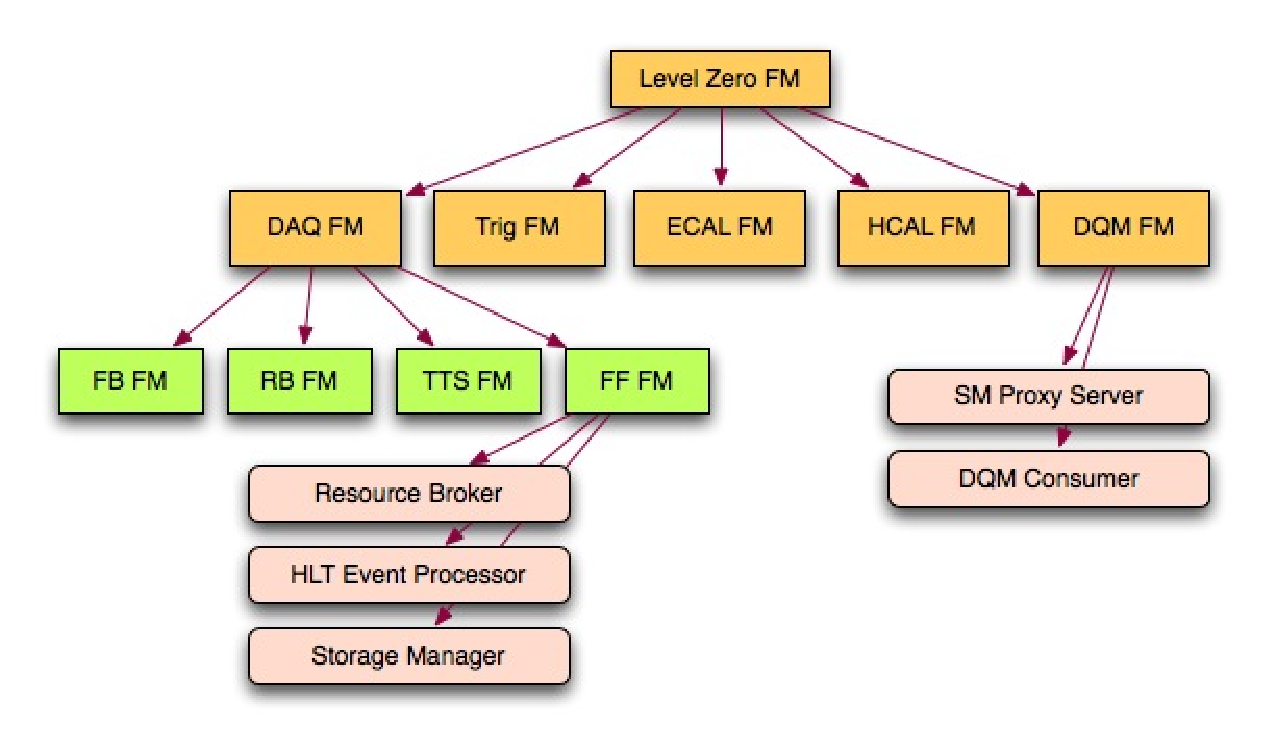
\includegraphics[width=4.5in]{Software/fm_example}
    \caption{Illustration of the hierarchy of Function Managers.}
    \label{fig:fm_example}
  \end{center}
\end{figure}

\subsubsection{Monitoring}

There are different levels of monitoring implemented for the Storage Manager
system, from the lowest level closest to the StorageManager and
SMProxyServer XDAQ applications, to higher levels where the monitoring
data has to pass through additional software.

Monitoring of the software at the lowest level is via the XDAQ application
console and the XDAQ application web pages. The console just contains text
that is output from the application. Different levels of text are generated
depending on their information content or severity, {\em i.e.} debug, 
informational, warning, and error levels. The text that appears from an
application can be filtered and also directed to specific consoles. These
text messages are created using the standard offline framework message logger
integrated with the online messaging system.

Each XDAQ application contains
a simple HTTP server that can serve web pages to a browser. The StorageManager
and SMProxyServer applications both have a number of monitoring web pages defined. 
These monitoring pages are dynamically generated when a browser requests
a specific web page. The monitoring pages include information on each HLT node
sending data like the node address, data rate, and latency. For the Storage
Manager itself, some information that is currently included are the status of the
XDAQ memory pool, the total maximum, minimum, and average data rate into and
out of the StorageManager, the average event size, the number of events received,
and statistics for the each streamer file written or being written. Other web pages
give the status of connected consumers and the status of the event and DQM servers.

Although a lot of information on the software status is available at the lowest 
level if needed, typically we minimized the processing the Storage Manager has 
to do to processes incoming web page requests. We make use of other monitoring
features of XDAQ. A list of important properties
of the Storage Manager is defined at configuration time and the Storage Manager
updates the information for this list. The list is accessible by other online
applications like the CMS Run Control. The values of the list of quantities are
published in the online XDAQ monitoring system and saved to a database from
which any number of applications
can access this information.

Standard web pages are generated using the monitoring lists for each XDAQ
application. Each online subsystem has a single web page summarizing the
status of that subsystem, called its ``Page One''. The Storage Manager Page One
has information mainly about the status of streamer files, and the status of
the output disk system. An example of the Storage Manager Page One is given
in Fig.~\ref{fig:sm_page1}.

\begin{figure}[hbtp]
  \begin{center}
    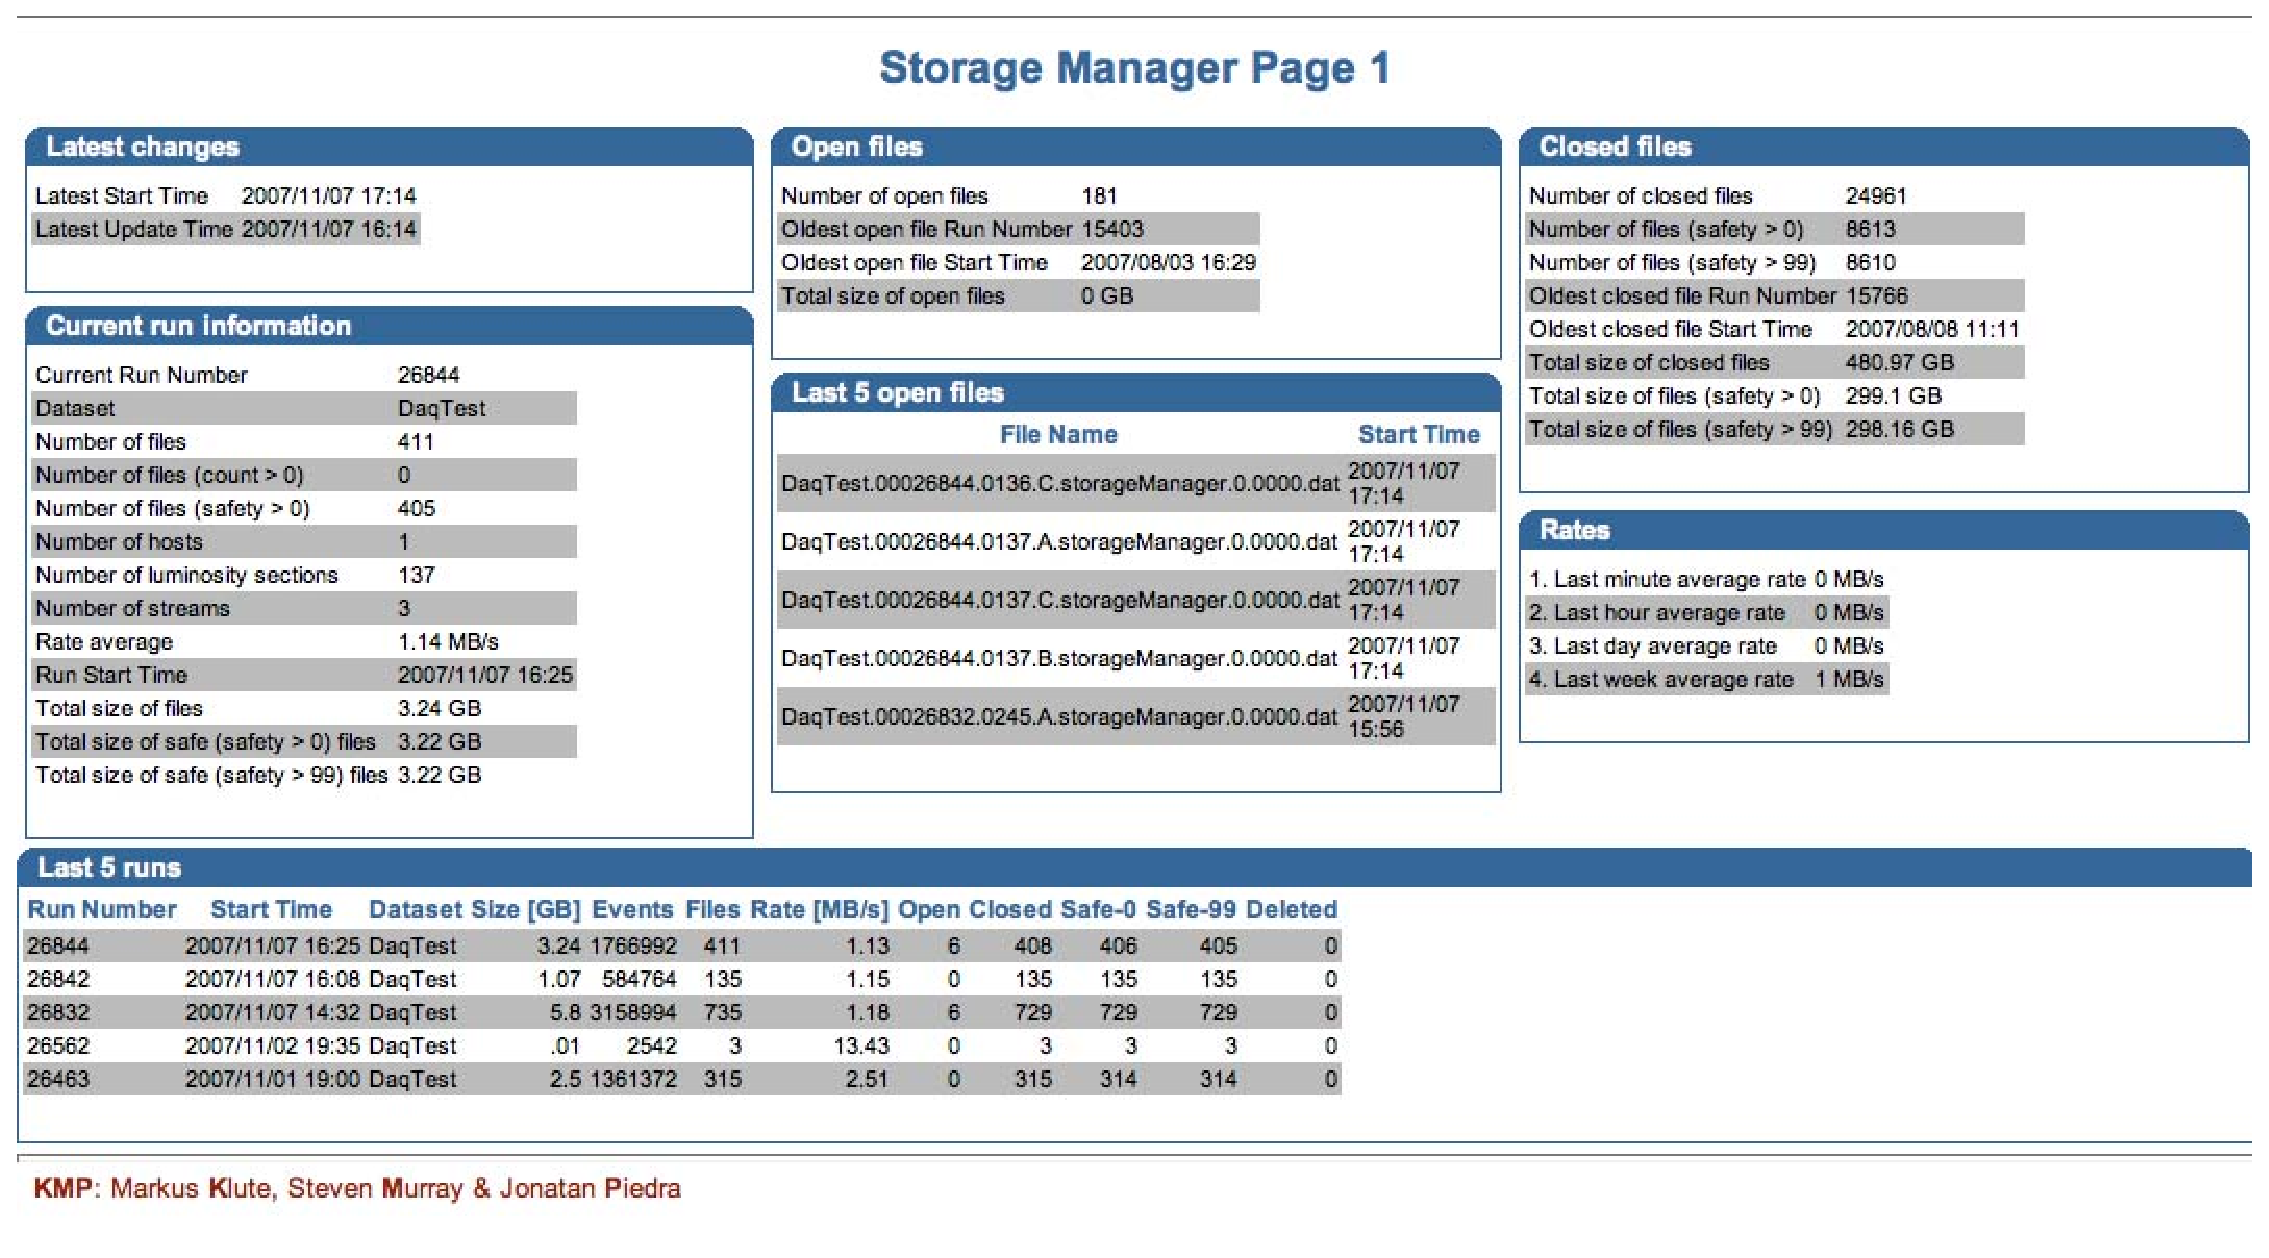
\includegraphics[width=5.5in]{Software/smpage1_example}
    \caption{Image of the Storage Manager Page 1 monitoring web page.}
    \label{fig:sm_page1}
  \end{center}
\end{figure}

The error alert system in the CMS online is still under development, and part of
the work of the SM group will be to integrate into this system when ready. In
addition the SM group is working on providing more monitoring and check-pointing
to help analyze problems that may arise, and to provide more useful information
for non-SM experts.

% The monitoring of the Storage Manager hardware will be covered in the
% hardware section.

\subsubsection{Error Handling}

There is currently some limited error handling in place for the Storage Manager,
mainly to handle the various error conditions so far experienced in the CMS global
cosmic ray data taking exercises. Handling of foreseen error conditions forms 
the major part of active code development for the Storage Manager group.
Currently most of the errors that are handled are considered fatal ones, and these
will cause the Storage Manager to go to the Failed state with an associated error condition 
message. Besides considering foreseen error conditions we have also received
experience from actual running of the system,
situations causing problems are analyzed and code changes for more monitoring
or error handling implemented if appropriate.

There are unit tests in place for the data serialization and deserialization code,
and for the streamer message creation and access. These unit tests are run during
each CMSSW pre-release and the production release to ensure that these code
function properly. The tests of the StorageManager and SMProxyServer applications
relies on a number of applications and already constitutes an integration test.
These tests are currently initially done manually on a test system consisting of two nodes.

The next validation tests are done on a CMS development system at the experiment,
the cmsdaqpreseries (Green Barrack) cluster. This system has installed the normal
CMS online with full Run Control and other features that enable tests of the SM system
software in a realistic online environment. The software development team has access
to this system and is being trained on operating it from Fermilab.
It is possible that many problems seen during 
data-taking can be reproduced in the cmdaqpreseries system and analyzed.
Currently scale tests and tests involving the actual SM hardware (disk arrays) are not
possible in the cmdaqpreseries cluster.
Scale and performance tests are done by the SM operations team on the actual SM hardware,
and a part of the CMS online system.

CMS has had a number of DAQ global run exercises and the Storage Manager is
an integral part of every global run exercise. The Storage Manager system is
scale tested up to the maximum foreseen rates
during these global exercises. Any problems or issues in each run
are diagnosed and corrected before the next global run exercise. Additional
functionalities or features of the Storage Manager may also be tested in the
global run exercises and in test running between these exercises.

Currently we are still collecting data on the types of error conditions we
face from the global run exercises, however we have created a  fault tolerant and 
error recovery policy. This policy is still awaiting feedback from the central DAQ group.
We will ensure that this error handling policy is an integrated policy that fits in with the CMS
online plan for fault tolerance and recovery.

Table \ref{tab:fc_errorhandling} gives the error handling policy proposed 
to the central DQM group.

\begin{table}
\begin{center}
\caption{\label{tab:fc_errorhandling}Error Handling Policy for Storage Manager 
Software Components.}
\vspace*{3mm}
    \renewcommand{\arraystretch}{1.5}
    \setlength{\tabcolsep}{2mm}
\begin{tabular}{| p{0.27\textwidth} | p{0.25\textwidth} | p{0.45\textwidth} |}
\hline
\multicolumn{3}{c}{\bf FragmentCollector} \\ \hline
{\bf Problem} & {\bf Cause} & {\bf Desired Reaction} \\ \hline
Corrupt data received from HLT such as invalid message types &
   Logic problems in upstream applications or memory corruption &
   Log error, keep statistics, discard fragment, (and all other fragments 
   for this event and output module). Keep running. \\ \hline
Unrecognized data (unexpected fragment type) & 
   Logic problems in upstream applications or memory corruption &
   Log error, keep statistics, discard fragment. \\ \hline
Missing fragments &
   Drop packets? &
   Provide timeout, log error, keep statistics, discard the partial event. \\ \hline
Out of order fragments & &
   Update the code to handle out of order fragments so that this is not a problem.
   Keep statistics � believe should not happen with tcp.\\ \hline
System exception &
   Exception thrown in a system call, or fatal error related to a system call, e.g. problem 
   writing to disk, no room on disk &
   Transition to a Failed state and log an error message. \\ \hline
Application exception &
   Exception thrown within the Storage Manager code. &
   For exceptions that are understood and can be handled, log them, keep statistics, and 
   discard fragment.  For exceptions which can not be handled, transitions to a Failed state 
   and log the error.\\ \hline
Incoming fragment causes application exception &
   Error decoding header, decoding DQM fragment with Root &
   Same as Unrecognized data (unexpected fragment type)\\ \hline
Event message view - bad protocol version & &
   Log error, keep statistics, discard fragment.\\ \hline
No event server &
   Logic error &
   Transition to a Failed state and log an error message? Or Just log error, 
   set monitoring alert and keep running?\\ \hline
Writer error & & See below\\ \hline
Wrong run number & Data from a mix of runs sent to the SM &
   [Update the code to determine the run number in a better way than from the cfg file.]  
   For events with the wrong run number, Log error, keep statistics, discard fragment.\\ \hline
Invalid fragment key &  & Log error, keep statistics, discard fragment.\\ \hline
Fragments in the queue after done message received & &
   Discard fragments, generate error message.\\ \hline
Could not stop writer properly & &
   Transition to a Failed state and log an error message.\\ \hline
Could not stop DQM event server properly & & 
   Transition to a Failed state and log an error message.\\ \hline
\end{tabular}
\end{center}
\end{table}

\begin{table}
\begin{center}
\vspace*{3mm}
    \renewcommand{\arraystretch}{1.5}
    \setlength{\tabcolsep}{2mm}
\begin{tabular}{| p{0.27\textwidth} | p{0.25\textwidth} | p{0.45\textwidth} |}
\hline
\multicolumn{3}{c}{\bf ServiceManager (writer)} \\ \hline
{\bf Problem} & {\bf Cause} & {\bf Desired Reaction} \\ \hline
Cannot write to a file & & Transition to a Failed state and log an error message.\\ \hline
Cannot create a file & & Transition to a Failed state and log an error message.\\ \hline
No space on disk & & Transition to a Failed state and log an error message. 
   Implement watermark alerts as disk partitions fill up.\\ \hline
Misconfiguration & & Transition to a Failed state and log an error message.\\ \hline
Event from closed lumi section (no test now) & & Log error, keep statistics, discard event.\\ \hline
Disk write too slow & & Log warning.\\ \hline
File move too slow & & Log warning.\\ \hline
\end{tabular}
\end{center}
\end{table}		
		
\begin{table}
\begin{center}
\vspace*{3mm}
    \renewcommand{\arraystretch}{1.5}
    \setlength{\tabcolsep}{2mm}
\begin{tabular}{| p{0.27\textwidth} | p{0.25\textwidth} | p{0.45\textwidth} |}
\hline
\multicolumn{3}{c}{\bf Event Server} \\ \hline
{\bf Problem} & {\bf Cause} & {\bf Desired Reaction} \\ \hline
Write to queue fails & & Log warning.\\ \hline
\end{tabular}
\end{center}
\end{table}

\begin{table}
\begin{center}
\vspace*{3mm}
    \renewcommand{\arraystretch}{1.5}
    \setlength{\tabcolsep}{2mm}
\begin{tabular}{| p{0.27\textwidth} | p{0.25\textwidth} | p{0.45\textwidth} |}
\hline
\multicolumn{3}{c}{\bf DQM Event Server and Service Manager} \\ \hline
{\bf Problem} & {\bf Cause} & {\bf Desired Reaction} \\ \hline
Deserialization of histo data fails & & Log error, keep statistics, discard the 
   offending DQM update.\\ \hline
Taking too long (too much CPU) & & Throttle somehow? \\ \hline
Disk write/file create/disk space (same troubles as other writer) & &
   Similar responses? Or log error and abandon DQM activities and keep running\\ \hline
\end{tabular}
\end{center}
\end{table}
		
\begin{table}
\begin{center}
\vspace*{3mm}
    \renewcommand{\arraystretch}{1.5}
    \setlength{\tabcolsep}{2mm}
\begin{tabular}{| p{0.27\textwidth} | p{0.25\textwidth} | p{0.45\textwidth} |}
\hline
\multicolumn{3}{c}{\bf TCP Transport (registry, data, DQM data, other)} \\ \hline
{\bf Problem} & {\bf Cause} & {\bf Desired Reaction} \\ \hline
Receive INIT message in wrong state (currently releases buffer, junks the message, 
   and keeps going) & 
   Additiional HLT processes started after the run has already started. &
   Transition to the Failed state? Or log error and keep running?\\ \hline
Invalid event selection in INIT (currently aborts, logs message)	 &
   Misconfiguration of HLT output streams &
   Transition to a Failed state and log an error message.\\ \hline
InitMsgView constructor fails - throw exception? & &
   Log error, keep statistics, discard fragment. Or transition to fail state because the 
   SM needs to parse the INIT message for checking configuration, etc.?\\ \hline
Receive event or DQM event data but not in run state 
   (currently release mem, discard data, log msg) & &
   Transition to the Failed state? Or log error and keep running.\\ \hline
Run number wrong (currently just releases memory) & &
   Log error, keep statistics, release memory.\\ \hline
Receive data from an unregistered FU & No INIT message sent &
   Log error, keep statistics, discard fragment.\\ \hline
I2O frame count is wrong (memory corruption) & &
   Log error, keep statistics, discard fragment.\\ \hline
Receive Other message but not in enabled state &
   Receive end of run when SM is not enabled &
   Transition to the Failed state?\\ \hline
Done from FU after Done from RunControl & &
   Transition to the Failed state?\\ \hline
\end{tabular}
\end{center}
\end{table}


\subsection{Status, Software Schedule, and Software Organization.}

The Storage Manager project started slowly in June 2005 with just two people
from Fermilab. The number of people in the Storage Manager group doubled with time
and the first prototype was produced for the Magnet Test and Cosmic Challenge (MTCC I)
in May 2006.
During this testing it was found that the deserialization step in the Storage manager was
too slow to write out ROOT output  files thus the decision was made to write out
the binary streamer files as a temporary format for use within the Tier-0 processing.

Another lesson learned was that the Storage Manager group needed a real presence
at CERN at the experiment during data taking. The MIT group joined the Storage manager
group and strengthened the group enormously in this area. 
The MIT group took over the operations
responsibility, including the interaction with Tier-0 and the hardware.

A second prototype Storage Manager writing streamer files was produced for MTCC-II
with more optimized concurrent writing to and reading from the disk system. The event
server functionality was commissioned during MTCC-II. Remote consumers were
served by an adhoc proxy server written to run on an Apache HTTP server.
The performance goals for the Storage Manager were met in MTCC-II.

The Storage Manager group was further strengthened with additional manpower
to finish the production version for the first CMS global run exercise in May, 2007.
An additional feature request of handling DQM data in the Storage manager was
taken and completed.
A series of performance tests in joint exercises with the Tier-0 team was done early in 2007
in preparation for the May global run exercise. The actual hardware for the SM system
was delivered in late in 2007, and performance tested in 2008. It was commissioned in the
March 2008 global run and in the Cruzet run in May 2008.
The SMProxyServer was commissioned in the experiment during the Cruzet global
run exercise in May 2008.

During the 8 global run exercises conducted so far the Storage Manager goals
were met and performed well. There were of course a number of small
issues and problems during the exercises, these have been fed-back to the
software development team.
The Storage Manager team were able to respond to problems
usually in a timely manner.

The schedule of software releases for the Storage Manager is govern by the
schedule of global run exercises and CMS Cosmic Runs (CCR) as well as
the actual start of collision data. The current schedule is to have Cruzet 2 in mid-June
and most likely another global run at zero field with the tracking system in the DAQ
before the CMS collision hall is closed for first LHC operations in mid-July.
Most of the future work for the
Storage Manager involves further commissioning of the
DQM data collection and summing, optimizing operation at the highest rates, improving
monitoring, robustness of the code and error handling. In additional documentation
of the Storage Manager will also be completed.

The Storage Manager team resident at Fermilab will continue to do the bulk of the
software development and code maintenance work, while the MIT team will continue to
be responsible for the interaction with Tier-0 including development and maintenance of
the code related to this task, with operations, and with the
Storage Manager hardware.


% $Id:$

\section{\label{sec:stohard}Storage Manager Hardware}  %Editor: Gerry

\subsection{Overview of Baseline System} 
An overview of the existing  Storage Manager (SM) hardware configuration 
is given in Figure~\ref{fig:system}. 
The HLT nodes are grouped in subfarms and connected to two (soon eight) 
gigabit ethernet switches (Force10). 
Data from the HLT is sent to 8 SM nodes (Loggers). 
%The input bandwidth is provided by 6 GigE links per Logger node providing. 
%Currently only 2 switches are connected with 2 GigE links to each Logger node.
% resulting in a total bandwitdh of 2GB/s. 
The Logger nodes are also connected to a GigE switch (Tier0) to provide connectivity 
to the Tier0 system at CERN.
The connection to the NexSan SATABeasts is provided through two Fibre Channel QLogic SanBox 5600 
switches. Each NexSan SATABeast unit has two controllers with two fiber connections. 
If one controller fails, traffic can automatically be switched to the second controller. 
The total network connectivity from the Logger nodes to the storage units is 8 time 2~Gb, 
such that the system is limited by the performance of the SATABeast controller. 
According to specifications each NexSan SATABeast should be able to reach up to $\sim$400MB/s write 
or $\sim$800MB/s read speeds, if equipped with a sufficient number of disks.
A system of 3 SATABeasts should be sufficient to meet a goal of 1 GB/s throughput,
and 6  SATABeasts the storage capacity goal.
However, the 8-fold symmetry of subfarms imposed by the connectivity 
of the 8 Force10 switches implies that efficient utilization of the subfarm resources
requires a multiple of 4 SATABeasts for balancing the load across the 8 subfarms.

% system overview
\begin{figure}[tbh]
\begin{center}  
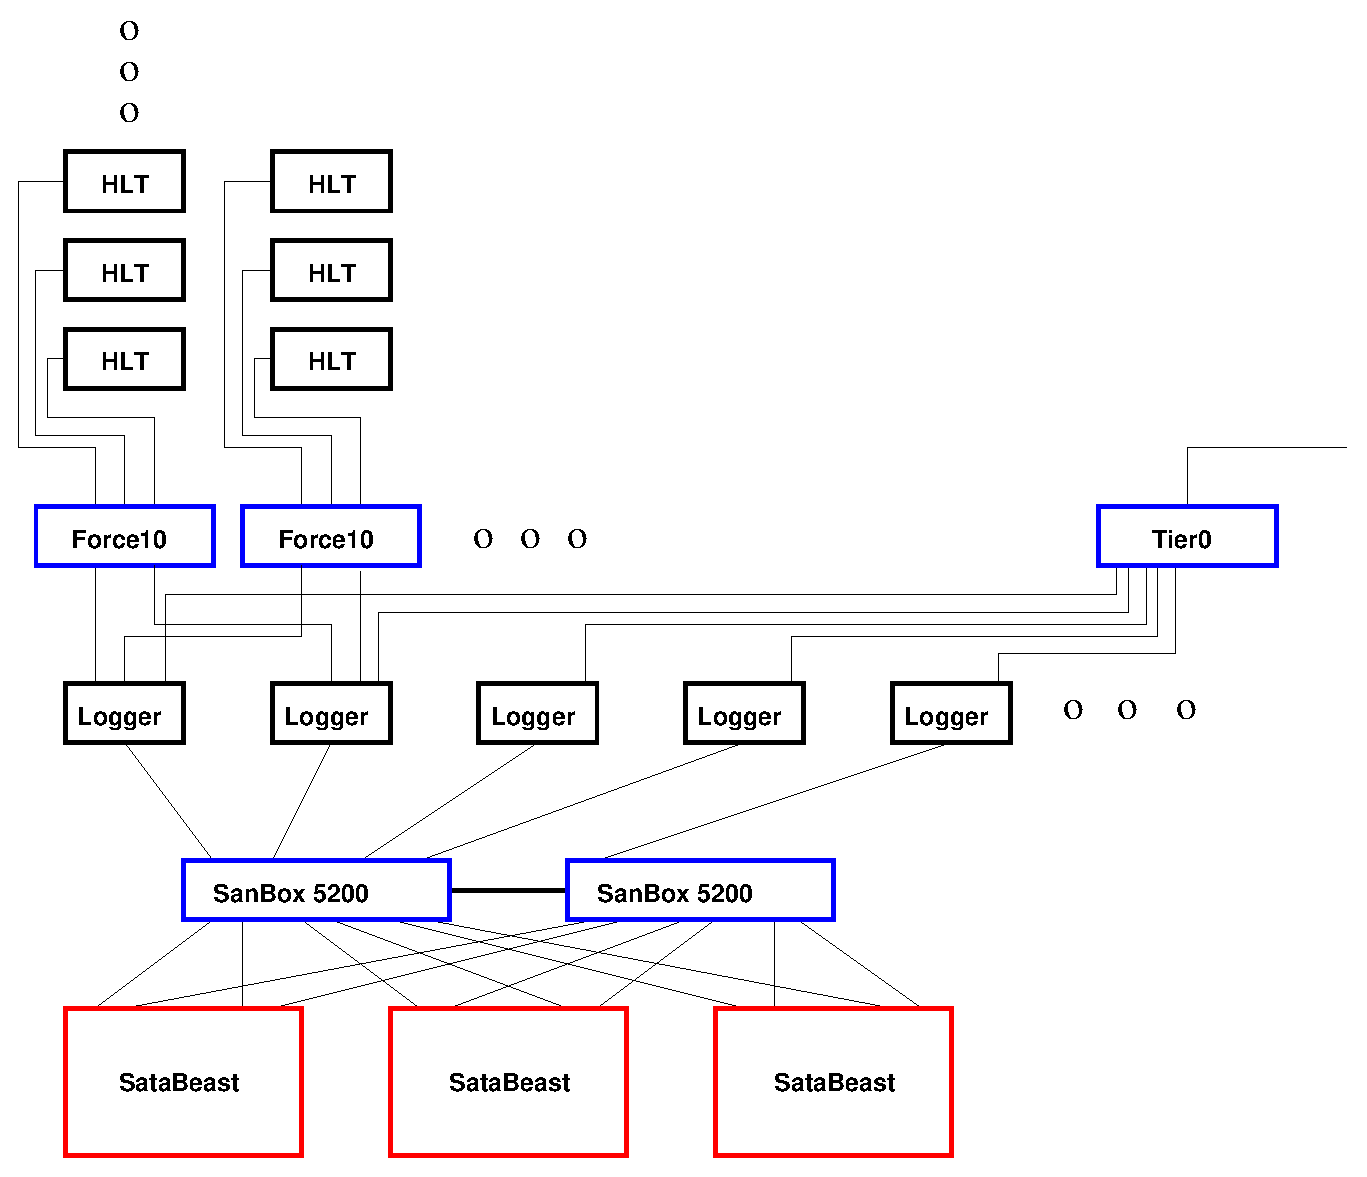
\includegraphics[width=1.0\textwidth]{Hardware/SMsystem}
\caption{\emph{ Storage Manager system overview of the currently installed hardware. 
The leftmost SATABeast is drawn indicating having the arrangement of four disk arrays, 
two arrays of which are ``owned'' by logger node 1 (``L1'') and two by logger node 2 (``L2'').}}
\label{fig:system}
\end{center}
\end{figure}  


\subsection{Hardware Components}
\subsubsection{Logger Nodes}
Logger nodes are standard Dell PC's PowerEdge 2950 with two dual-core Xeon processors and 4 GB RAM. 
Each node is equipped with a 4-port GbE card (Silicom PEG4i) and 
a fiber channel host bus adapter (QLogic QLE2460-CK). 
% An additional PCI-e slot is available for an extra 4-port GbE card if needed. 
The same PC's are used for the CMS HLT farm.
The SM nodes are fully incorporated in the DAQ group's Quattor system for managing 
the software installation of PCs.

\subsubsection{Fiber Channel switch}
The fiber channel switches are used to connect the logger nodes and the storage. 
Two QLogic SanBox 5600 switches are used. 
Each chassis includes sixteen 4Gb ports, plus a four-pack of high-speed 10Gb ISL ports 
of which one is used to connect the two switches.
The latter interconnect can be used to re-route traffic through the other switch
to reconfigure around the hardware failure of certain components.

\subsubsection{Storage Array}
The storage arrays are the SATABeast from NEXSAN. 
Each SATABeast has two controllers with two 2~Gb ports.
The total number of disk slots available is 42 and the system can support Sata disks 
of up to 1~TB size. 
NexSan SATABeasts have been successfully deployed for the CDF Consumer Server Logger system 
at Fermilab since 2006.

The arrangement and allocation of disks in the SATABeast is constrained by a number
of practical considerations.
Without substantial investment in a file management system it is simplest
to dedicate disk arrays to particular logger nodes, and given our use case, 
there is not much incentive to overcome this choice.
Due to its dual controllers, the SATABeast is best fed by two logger nodes,
implying a division of the SATABeast into an even number of disk arrays.
Given the  SATABeast capacity is for 42 disks, and one wants hot spares, 
the obvious choice is a configuration of four 10-disk arrays plus 2 hot spares.
By giving each logger node write control of two arrays, one can also obtain some benefit
from reading and writing from separate arrays, even though we do not plan
to enforce non-overlapping I/O. We can envisage such a scheme if it is warrented.
The 10-disk arrays are also appropriate in that much smaller arrays would
suffer reduced throughput; and dramatically larger arrays would be at greater
risk for multi-disk failures, and longer re-build times.
The size of the disk arrays can be an issue for some file systems, 
but partitioning the arrays with multiple volumes easily avoids such limitations.


\subsection{Storage Manager Performance}
The prototype system, currently installed in Cessy, has
3 SATABeasts installed  with 10 Sata disks of 750~GB  and 116 of 1~TB.
These are currently configured in our baseline in groups of 10-disk RAID5 arrays 
(2 spare RAID disks per SATABeast), yielding an effective capacity of 105.75~TB storage
for the full system.
With the dual controllers, a single SATABeast is expected to be fundamentally 
limited to about 400 MB/s writing.

The HLT subfarms are connected via a FORCE10 switch through
two 2~GbE Silicom links (``rails'') per logger node.
Presently the DAQ system is being recabled for the full contingent of eight FORCE10 switches
such that each switch, corresponding to a DAQ ``slice,'' has connectivity with 
a single SM logger node.
Another layer of a pair of additional switchs are being contemplated by the DAQ group
that would remove this restriction.
The Ethernet connection limits the theoretical wire-speed of data input
to a logger node to 250~MB/s.

Each logger node is connected to the Tier0 switch with a single 2~GbE link.  

The 3-SATABeast prototype system was designed to be able to provide a throughput of about 1~GB/s,
but it falls short of the design of 250~TB capacity. 
This requires an expansion of the system, which is discussed in Section~\ref{sec:SMexpansion}.
Because each SATABeast will collect the data from two DAQ slices, and the slice structure
is simple replication of parallel structures, a single SATABeast fed by two logger nodes
is the atomic unit for projecting throughput performance---although we usually quote
results on a per node basis, test numbers are
obtained using two nodes each accessing a seperate disk array unless otherwise stated.
We use this model in our performance studies and extrapolation to that of the full system.

The nominal setup for our system tests include the following features (unless stated
otherwise):
\begin{itemize}
  \item SLC4 Linux installation on logger nodes
  \item 2 logger nodes accessing separate ten-physical-disk arrays on the same SATABeast
  \item Each logger node has control of two arrays, and alternates the file writing
between these two arrays as luminosity sections are incremented
  \item 128k SATABeast stripe size (max allowed)
  \item RAID5 disk redundency
  \item XFS file system on the SATABeasts
  \item Single output stream
  \item $\sim$1 MB event size
  \item 1 GB data file size 
\end{itemize}
Our tests can be categorized in terms of subcomponent capability and full system tests.
Subcomponent tests include:
\begin{itemize}
  \item {\bf Ethernet Input on Logger Nodes:} The Ethernet throughputs have been tested for two cases.
First, we have set up the full DAQ readout chain but flagged all the data from FUs to the SM
to be a stream that is {\it not} written out. In this case a 1-rail SM sinks about 110 MB/s,
and a 2-rail SM takes in 220 MB/s.
Similarly, the single logger-node link to Tier0 for simple file transfers (with no other activity)
also saturates  at about  110 MB/s.
  \item {\bf Direct Logger Node Write/Rread to a SATABeast:} To gauge the write performance 
from a logger node to a SATABeast 3 GB files were generated by \verb+dd+ (64k block size)
and written to a  SATABeast disk array; read tests were done with 1 GB files. 
Early tests with few disks provided rather low rates, but
later we settled on 10-disk arrays as a compromise configuration. 
We obtained the following results:
%\begin{table}[h]
\begin{center}
\begin{tabular}{c|c|c|c}
\# nodes   & \# Arrays & Write Only (MB/s) & Read Only (MB/x) \\ \hline
1          &     1     &     198           &    211\\
1          &     2     &     198           &    200\\
2          &     2     &     377           &    383\\ \hline
\end{tabular}
\label{tab:ddrates}
\end{center}
%\end{table}
With two logger nodes we have driven the SATABeast near the expected 400 MB/s maximum.
Similar performance was seen with \verb+dc_bench+.

The choice of 10-disk arrays is, as much as anything, almost a forced choice
given that that the SATABeast is limited to 42 disks and at least 2 disk spares
seems to be a minimum choice, and one would like an even number of arrays.
However, in terms of \verb+dd+ write rates, 10 disks is also a good choice:
\begin{center}
\begin{tabular}{l|c|c|c|c|c} \hline
\# Disks:      &   6    &   7    & 8    & 10   &   13\\ \hline
Rate (MB/s):   & 160    & 174    & 180  & 198  &  200\\ \hline
\end{tabular}
\label{tab:ddrates2}
\end{center}
  \item {\bf Data Transfers to Tier0:} We have tested reading data files from
a  SATABeast via logger nodes and sending them out through a single  2~GbE link
to Tier0.
Dedicated read-only from the SATABeast, and using the standard \verb+CopyWorker+
transfer scripts, saturates the Ethernet at about 100 MB/s per logger node.
\end{itemize}


We can put all the pieces together in full system tests, 
which run the standard SM executables
and employ the full DAQ chain beginning from one or two crates of FRL's,  
run in a  mode where data was internally generated,
and have these event fragments built by the normal chain of RU's and BU's,
then feed to FU's, and finally
pass the events to the SM for recording over two Ethernet rails.
The filter algorithm of the FU has data  compression turned off and 
the event size was padded with dummy arrays to make it about 1 MB.

The operation of the SM consists of a series of stages which can be
functionally subdivided as:
\begin{enumerate}
  \item SM Receiving and handling events from the FU  
  \item SM Writing events to disk (each logger node alternates between writing to two of its own  arrays)
  \item For each file written: database operations for file bookkeeping and for the transfer system 
        are done by the SM executable
  \item Actual DB operations and transfer process of files to Tier0 are done by independent scripts
        (not by the SM executable) 

\end{enumerate}
The throughput rates measured for various permutations of these processes being
active or not in full DAQ running  are (in MB/s):
\begin{center}
\begin{tabular}{c|c|c|c|c|c} 
2. Write Files & 3. DB actions & 4. Transfer to T0 & SM Throughput  & Tier0 Rate& SATABeast Throughput  \\ \hline
   NO       &   NO       &    NO          &       220      &   --- &   ---       \\
 {\bf YES}  &   NO       &    NO          &       180      &   --- &   180       \\
 {\bf YES}  &  {\bf YES} &    NO          &       144      &   --- &   144       \\
 {\bf YES}  &   NO       &   {\bf YES}    &       150      &    50 &   150$+$50  \\
 {\bf YES}  &  {\bf YES} &   {\bf YES}    &       150      &    50 &   150$+$50  \\
\end{tabular}
\label{tab:rates}
\end{center}
These rates are quoted on  a {\bf per logger node} basis, although the measurements
were actually performed with two logger nodes feeding a single SATABeast.

It is interesting that there is a noticeable, and equal,  penalty for DB actions
and for transfers to Tier0, but one seems to ``shadow'' the other.
Also note that these test were done with the DB access managed by perl scripts invoked
by the SM executable. We have been in the process of restructuring this whereby
the DB access is entirely decoupled from the SM executable (see Section \ref{sec:fpt0}).
This may reduce the overhead delays in the SM from DB access.
We do not, however, count any performance improvement from this change.
This example highlights the fact that other fine-tuning of the system may be possible
and profitable for improving SM performance, but we note that this does not appear 
to be actually necessary for the SM to meet our original goals.

A further teasing apart of the effects on throughput is seen in an early
test with two SM nodes writing two arrays on a SATABeast, of 6 and 7 disks respectively,
that gave a rate of about 140 MB/s writing 1 GB files (no reads).
When each node was reconfigured to write the output in a {\it single} file of unlimited
size the rate increased to about  150 MB/s.

Questions about CPU load can only be fully addressed with all functionality
in place, including the eventual DQM load.
Howerver, a rough look at the \verb+top+ load when running the full DAQ chain and
transfers to Tier0 indicate the CPU is occupied $\sim$15-30\% by the system plus ``users,''
$\sim$20-50\% in I/O wait, and $\sim$20-80\% idle.
No problem is apparent at this point.
Heavier demands from additional tasks could change this picture, 
especially motivating an expansion of PC memory.

A variety of miscellanous issues were investigated with respect to throughput rates:
\begin{itemize}
  \item {\bf File Systems:}
Our initial choice for the file system was XFS.
However, during heavy loading with \verb+dd+ tests, and relatively rare incidents 
in full DAQ running,
we observed the logger nodes crashing (log messages indicated paging problems).
We tested a Linux kernel build under SLC5, and did not observe this problem.
However, operating with what is at this point non-standard software is not 
viewed as a very practical option.
We also configured the SATABeast file system under Ext3, and again did not observe
this problem.
In fact, most of the May Global Run (CRUZET-1) was run  with  Ext3
without any SM incidents.
We need to still be sensitive to possible negative impacts of choosing  Ext3 over XFS,
but so far we have not uncovered any major downside with running  Ext3,
and we have now adopted it as our default system.

  \item {\bf Multiple Output Streams:}
We have done a prelimiary test running the full DAQ chain to the SM with 
up to 5 output streams so far.
Interestingly the throughput performance showed a small increase 
in rate to 192 MB/s (compared to the benchmark of 180 MB/s).
When running with even more streams we ran into reliability problems
with the XFS file system (previous bullet).
These tests need to be extended with Ext3, but indications so far are
that multistreaming is not an issue.

 \item {\bf Large Number of Socket Connections:}
As a practical matter the SM is so far usually run with either a small number of FU's 
or  low throughput, and thus  one has  not been sensitive to the impact on performance 
of a SM node having to manage a large number of socket connections.
For 2008 LHC running the DAQ system expects to be running about 720 FU's---one
\verb+EventBroker+ (i.e. one socket connection to the SM) each.
With a 16-SATABeast system each logger node would support 45 FUs,
and any eventual system doubling would only push this 
to 90 FUs per logger.\footnote{Because of the finite rack space available, 
the DAQ group is significantly constrained that future increases of the filter farm take 
the form of larger numbers  CPU cores per FU rather than proliferating physical boxes.
This implies that even dramatic increases in CPU power of the filter farm
should not have a large effect on the connection load of the logger nodes.
Although, future upgrades with more rails is a possibility, but the capability
of the logger nodes would also presumably be improved.}
We ran a large connection test by feeding the output of 100 FUs into
a single SM (Ext3 file system, no DB actions, and no Tier0 transfers) and
achieved the usual write rate of 180 MB/sec.
An even larger system of 300 FUs showed only a modest drop to 150 MB/s.
\end{itemize}


Our essential conclusion is that while there may be worthwhile optimizations 
of the system, these results with one SM ``leg'' demonstrate that we are on track
to meet our performance goals even with the {\it existing}
state of the hardware and software.


\subsection{Hardware Expansion\label{sec:SMexpansion}}

The initial prototype system assembled in late 2007 was envisaged as Phase-I 
of a three phase expansion, the later phases were primarily to increase the
storage capacity.
Phase-II was to increase the disk inventory by 96 disks to fill up the existing
SATABeasts in the spring of 2008.
Phase-III was forseen for 2009 to essentially double the system for higher 
luminosity LHC running.
We have been operating under the general philsophy of this plan, 
but two developments have modified its execution.

First, we found that our testing of the system and providing support for CMS
running with a portion of the new SM hardware was, or would be, significantly hampered 
by the small inventory of disks on hand.
In particular, high data rates to the SATABeast is conditional upon have
fairly large disk arrays.
Therefore the Phase-II disk purchase was accelerated by a few months,
giving us in early April the 118.5TB currently installed.

Second, CMS management in consulatation with DAQ and trigger
project managers concluded that the doubling the system in 2009 would be
better done  for the 2008 LHC run.
Essentially, in this early phase where operation may be unstable 
for the accelerator (e.g. store frequency)
and detector (e.g. triggering, zero-suppression,\ldots), 
it may be very important for CMS to be able to maximize  recording very high data rates
for the limited store-hours available.
The SM hardware team  was thus asked in May to quickly pursue doubling the system.
We have begun the process for purchasing the requested doubling, 
but have also incorporated two secondary design changes.

First, by virtue of the connectivity of the eight FORCE10 switches, the DAQ system
will have an explicit eight-fold symmetry in the data flow.
By having 8 logger nodes, the front end of the SM system is properly matched,
however, 8 nodes feeding 3 SATABeasts is not---the 8 nodes were originally 
conceived as 6 loggers $+$ 2 spares.
The SATABeasts are able to support eight slices,
but doing so breaks the natural topology of one node per  SATABeast controller.
This has the important impact that having 8 rather than 6 nodes will umbalance 
the throughput that the filter farms 
can support, and  the large investment in filter computing resources would be underutilized.
Thus the decision that the  SATABeasts should properly match the 8-fold symmetry
of the greater DAQ system, and that the prototype  configuration should consist
of four  SATABeasts rather than three.


A second modification of the design concerns the robustness of the system.
The Fiber Channel switches that move data from the logger nodes to the 
SATABeasts are fault tolerant, and allow traffic to be routed from one
switch to its partner and still make it to all SATABeasts. 
However, we have already experienced a failure of a switch {\it power supply}
and lost the connections for four of the logger nodes to the  SATABeasts.
To improve fault tolerance the expanded system will equip the logger nodes
with two Fiber Channel connections, one to each switch, so that complete failure of a switch
will not interrupt operation.

Aside from these two alterations, the system expansion is then a simple doubling,
and the final system for 2008 data taking should consist of:
\begin{itemize}
\item 16 logger nodes $+$ 2 hot spares
\item 4 Fiber Channel switches $+$ 1 pre-configured spare
\item 8 SATABeasts fully loaded with 42 disks
\end{itemize}
This system should readily exceed the original throughput/storage goals.

Assumming the purchase process and equipment delivery proceeds in a timely
fashion we would hope to have the full system in operation by the fall.


\subsection{SM Commissioning\label{sec:SMcommiss}}
The Phase-I system was installed in the latter part of 2007.
Performance studies were begun in Dec 2007 and carried out through the spring of 2008.
In Feburary 2008 the Tier0 connection was commissioned.
With the arrival of the supplementary disks (Phase-II) a SATABeast was configured
and ``delivered'' to the DAQ group in April for their routine use,
i.e. both for generic DAQ system tests and CMS data taking, especially for Global Runs.
This 1-SATABeast system includes two logger nodes, each assigned two 10-disk RAID5
arrays.

This 1-SATABeast system, in conjunction with the old MiniDaq SM which we continue
to support, has been more than adequate to serve CMS data taking needs.
We prefer to operate with the other two SATABeasts reserved for SM testing
and development, but on short notice, or for special purposes, we can devote
a second, or even the third SATABeast for CMS use.
Thus we are well positioned to support CMS needs.

In the short term future, conducting more realistic full-scale testing
is somewhat problematic from a variety of perspectives: 
the full DAQ system is not in place, 
and there is considerable demand for its resources purely from among DAQ developers;
a realistic data profile and final HLT algorithms are not in place;
and the DQM related impact upon the SM is not known as it is still under development.
We see meaningful large scale system tests of the SM will increasingly be integrated
within the context of overall large scale DAQ testing.

 
Installation of the hardware for the SM expansion (Sec.~\ref{sec:SMexpansion}), 
assuming a rapid procurement process, should take place by the fall.
The physical installation of the new hardware is essentially a duplicate
system in a neighboring rack, and the assembly and commissioning work
would nominally be done with no interference of the existing system.
The exception is the 4th SATABeast to be installed in the old rack,
and installation of a second Fiber Channel port on the existing PCs.
This may in fact require some reorganziation of the existing rack, 
or at least presents a good opportunity to do so.
Ideally we would commission the new rack before embarking on any major
disruption of the old SM rack, but in any event, we would seek to maintain
at least one data-ready SATABeast at all times.
Our goal would be to have the entire expanded SM system operational
in early September.


\subsection{Personnel Support for Hardware Commissioning and Operations}

At the time of the last review, in Nov 2007, the MIT hardware team 
was undergoing major personnel changes.
This centered around the then immenent departure of Markus Klute
to a faculty position, and the review committee expressed
some concerns as to the adequacy of human resources.


In late November, Research Scientist Gerry Bauer joined the SM project
full time, and thesis student Matt Rudolph joined part-time while still maintaining
activities in the tracker group.
A search was begun for a relacement of Klute, and this gap was
filled in March 2008 with the addition of Constantin Loizides,
a physicist with IT training, to the  MIT SM team. 
In early June the MIT team will be further enhanced by the addition
of Josep Serrano, an IT professional, as System Administrator.
Christoph Paus continues his leadership, now as a formal USCMS 
L-3 project co-manger along with Harry Cheung.

In summary, MIT maintained continuous personnel support of the SM hardware project 
through the departure of M. Klute, and further expanded the level of support
commensurate with the enlarged system.
We are confident that we have the necessary personnel to meet SM commitments,
and that the initial cautions expressed by the reviewers 
has been well addressed.


\subsection{Hardware Cost and Future Projections}
Table~\ref{tab:proto} shows the costs for the proto-type system purchased in 2007 
with the exception of the Logger nodes, Silicom cards and fibers, 
which where ordered together with the nodes used for the HLT farm or a database project,
and supplied by CERN. 
In total \$80k were spend on the proto-type system. 

A cost summary for hardware through 2010 is summarized in  Table~\ref{tab:costs}.
It includes the expenditures for 2008, which are either completed
or based on quotes supplied by vendors, except for an year old estimate 
for optical fibers.
The 2009 and 2010 projections costs are based on current costs,
with no attempt to account for falling technology prices or inflationary increases.

No new major purchases are forseen for 2009 or 2010, 
however, warrenty periods will be expiring, and in particular our original
three SataBeasts will go off warrenty in 2010.
Hardware failures are of course unpredictable, but we have separated
our estimates in terms of `disks' and 'Misc. Hardware' as  statistical
projections of disk failures are more meaningful with our large sample.
The funds listed under ``Misc. Hardware replacement'' would be sufficient
for one major sub-component failure (e.g. $\sim$\$5k for SataBeast controller) and
still leave a small reserve for other small component failures.
This division is of course only conceptual, and
actual experience will dictate the ultimate allocation of funds for replacement 
hardware.

\begin{table}[!ht]
\begin{center}
\begin{tabular}{l|r|r}
year & cost    & product \\\hline\hline
2007 & \$66k   & 3 SataBeasts with 10 disks  \\\hline
2007 & \$6k    & 2 QLogic switches$+$hardware  \\\hline
2007 & \$8k    & 8 QLogic HBAs \\\hline
2007 & \$4k    & 2 QLogic switches hardware \\\hline
2007 & CERN    & 8 Dell PowerEdge 2950 PCs\\\hline
2007 & CERN    & 8 Silicom PEG4i \\\hline
2007 & CERN    & 20 2m fiber \\\hline\hline
\end{tabular}
\caption{Prototype system costs.}
\label{tab:proto}
\end{center}
\end{table}

% Second Fibre Controller (2 fibre and 2 iscsi ports) Pricing $4,922
% FC switch: ~3k

\begin{table}[!ht]
\begin{center}
\begin{tabular}{l|r|r}
year  & cost      & product \\\hline\hline
2007  &     \$80k & prototype system \\ \hline\hline
2008~~Feb&  \$46k & 100 1TB  SATA disks  \\\hline
2008~~May& \$182k & 5 SataBeasts with 42 disks  \\
         &  \$11k & 25 Spare 1TB SataBeasts \\
         &  \$16k & 2QLogic switches$+$hardware  \\ 
         &  \$25k & 20 QLogic dual HBAs \\\hline
2008     &   \$1k & 50 2m-optical fiber \\\hline
2008     & CERN   & 10 Dell PowerEdge 2950 PCs \\\hline
\hline
2009     &  \$11k & 25 Replacement 1TB disks \\ \hline
\hline
2010     &  \$11k & 25 Replacement 1TB disks \\ \hline
2010     &   \$7k & Misc. Hardware replacement  \\  \hline
\end{tabular}
\caption{Storage Manager system costs to 2010.}
\label{tab:costs}
\end{center}
\end{table}

%% 
%% \begin{table}[!ht]
%% \begin{center}
%% \begin{tabular}{l|r|r}
%% year & cost    & product \\\hline\hline
%% 2007 & \$80k   & proto-type system \\\hline
%% 2008 & \$51k   & 96 SATA disks  \\\hline
%% 2009 & \$66k   & 3 SataBeasts with 10 disks  \\\hline
%% 2009 & \$51k   & 96 SATA disks  \\\hline
%% 2010 & \$17k   & Hardware replacement  \\
%% 
%% \end{tabular}
%% \caption{OLD:: Storage Manager system costs.}
%% \label{tab:costsOLD}
%% \end{center}
%% \end{table}
%% 
%% 

%% memory expansion??

% Operations Plans
\section{Storage Manager Operations\label{sec:SMoperations}}

\subsection{Operational Experience \label{sec:SMexperience}}

Throughout 2007 we supported CMS development, commissioning, and data taking
with the small provisional SM systems (\verb+cmsdisk0+ and \verb+cmsdisk1+).
This has continued in 2008, however,
since March a dual-node$+$SATABeast system has been dedicated
as the mainstay of CMS data taking.
We prefer to reserve the other two SATABeasts for technical development
and testing, but as the need arises we can quickly integrate one, or both,
of the other SATABeasts into normal CMS operations---it is largely and 
administrative decision.

As an example of the use of the SATABeast by CMS,
the data throughput for the ``CRUZET'' Global Run is shown in Fig.~\ref{fig:cruzet}
for the two logger nodes.
Not surprisingly, cosmic ray running does not push the system very hard.
Operationally, once things are in place the Global Runs for the SM have
generally been smooth.
The run usually begins with a new, or even changing, software release,
and this means some setup issues are not always correct.
Once these are worked out, the SM running has been smooth except for one incident.
We began CRUZET using XFS (nodes 19 \& 20), and this seemed to caused a number
of incidents of node crashes.
Once we switched to Ext3 (nodes 15 \& 16), which is most of the data, 
no further SM problems were reported.

% cruzet
\begin{figure}[t]
\begin{center}  
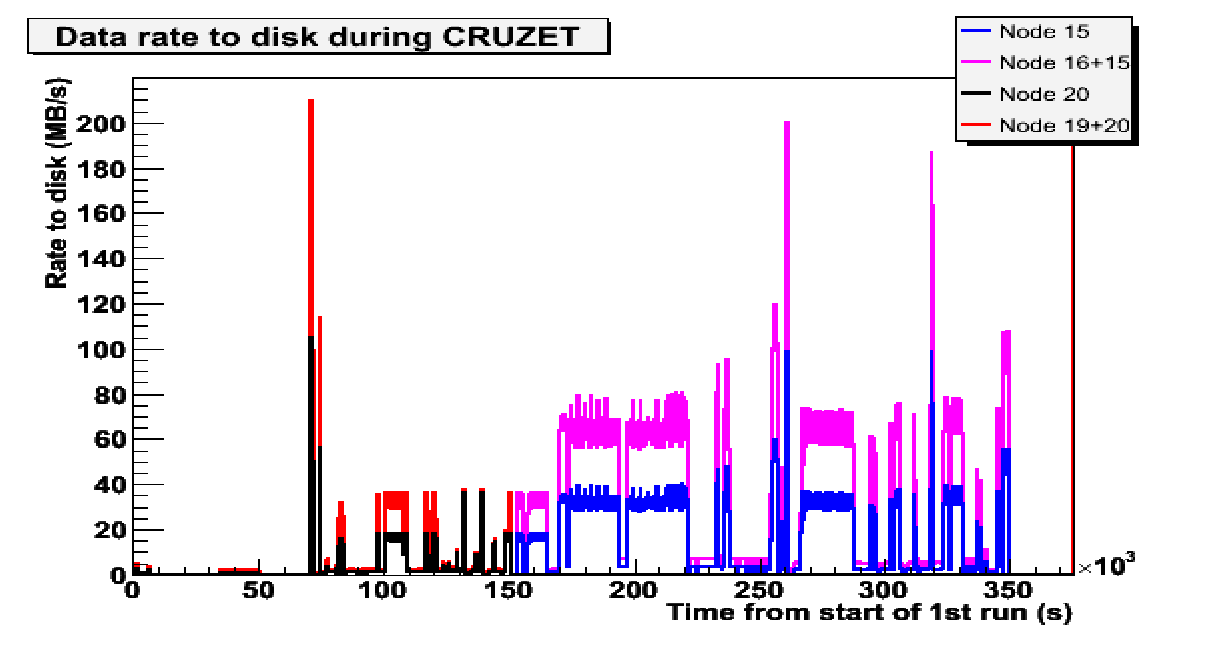
\includegraphics[width=0.9\textwidth]{Hardware/cruzetByNode}
\caption{\emph{Storage Manager throughput during the May 2008 ``CRUZET'' Global Run. 
The SM in CRUZET consisted of two logger nodes each running two SM instances,
thus making up a 4-Slice DAQ configuration; and the two logger nodes wrote
to a single SATABeast with 4 ten-disk arrays.
 The Global Run began with Nodes 15 and 16
writing to a single SATABeast with 4 disk arrays with the XFS file system.
Later in the run we switched to Nodes 15 and 16 writing to a SATABeast withh the Ext3
file system.
The lower traces are the throughput of one of the two nodes
(either 15 or 20), and the upper trace is the the total through put for
the two nodes (either 15$+$16, or 19$+$21). 
The SM used only a single ``rail'' each, and thus the spikes are reaching the network 
maximum of about 220 MB/sec total throughput. The spikes are brief occurances
due to trigger tests or improper trigger settings, 
i.e.  trigger rates for meaningful cosmics do not drive such high data rates.}}
\label{fig:cruzet}
\end{center}
\end{figure}  

For operation of the expanded SM system, we
would hope that timely processing and delivery of the new
hardware (Sec.~\ref{sec:SMexpansion}) would allow the full system 
to be in operation in September. 


\subsection{Response Plans for Hardware Failures \label{sec:SMhardfail}}

In order to minimize or avoid system down-time we envisage the following
sorts of protection against hardware failures.

\begin{itemize} 
\item {\bf Logger Node Failure:} We plan to pre-configure 2 PCs as ``warm'' spares.
The PCs would be equiped and tested with the full networking capability.
Due to the lack of spare ports for the switches, and the fact that
a preconnected spare that is truly ``hot'' will have a new identity
that would require a new DAQ configuration to be made (an expert activity),
it is deemed preferable to have ``warm'' spares which have been tested
to have full functionality, but to have them assume the host name of the
failed logger node via a Quattor system installation.
Since all DAQ PC's are administered via the Quattor management system
it is quick and easy (but still an expert action) to install a new PC with
the identity of a defunct node.
Then in addition to moving a few cables the spare node would fully assume
the old identity and be completely
functional in the existing DAQ system configuration. 

\item {\bf Fiber Channel Switch Failure:} The Fiber Channel switches have 
their own level of fall-over protection, in particular, traffic can
be rerouted to the partner switch.
However, catastrophic failures, like a complete power supply failure
can still bring down the switch.
Therefore are plan is to configure the expanded system with 2 fiber links
from each PC, one of which will be connected to each switch.
The SATABeast already has this dual connection split over the two switches.
This will then enable a complete and utter failure of a fiber channel
switch without impacting operations.
Furthermore, in the enlarged system with 4 switches in use, we plan to
pre-configure a hot spare switch which will only require moving optical
cables in order for it to take over from the failed unit.
Parenthetically, we note that this spare would also be of utility
in the event of a fiber channel switch failure in the CMS DB
installation at Cessy,  which has no spare in-hand.

\item {\bf SATABeast Controler Failure:} A part of the standard SATABeast 
design is the ability to be configured such that if one controller fails the second 
one can pickup the traffic without interruption.
We have not yet tested this feature, or seen the performance impact.
However, as each controller will only be supporting 1/16 of the data flow,
this should not have a dramatic impact.
We are investigating the particular procedures and response times
for Nexsan to provide replacement parts.

\item {\bf SATABeast Disk Failure:} The purpose, of course,
of the RAID array is that a disk may fail without loss of data.
Our baseline  mode of operation is to run RAID5 which will tolerate
a single disk failure.
Depending on the expectations of data demands, and experience with failures,
we may consider RAID6, allowing two disk failures in the same array.
With our division of four 10-disk arrays, and 2 hot spare disks,
and an assumed disk failure rate of 5\% per year, one in fact expects
to replace 2.1 disks per year per satabeast.
In a 3-day period (eg over a weekend) there is about 1.6\% average probability
of a single disk failure out of 40 disks---assuming uncorrelated Poisson statistics,
this drops to $1.3\times 10^{-4}$ for two or more disks failing in that 3 day window
(not necessarily in the same array).
RAID5 operation seems well warrented for these average statistics.
However, as disks age this average estimate may be too optimistic,
and a more mature system in later years may warrent revisiting these numbers.

A disk failure does not lose data, but could yet impact performance.
We exercised the RAID rebuild function of the SATABeast to understand the
impact on data rates.
Rebuild times are quite substantial, and depend on array size and the rebuild 
Priority setting. A small 4-disk array rebuilds in 8.4 hours for the highest
priority, and 11.1 hours in the lowest priority---all with no other activity on the SATABeast.
A 10-disk array takes 13.3 hours at the highest priority.
We started a run of the full DAQ chain to a single logger node 
to a single SATABeast array and were obtaining stable write speeds 
(no transfers or DB activity) 
of about 194 MB/sec (writing to a single array with XFS), 
and then triggered a simulated  disk failure {\it during} the run.
The write speed only decreased to 188 MB/s, but the rebuild rate dramatically increased.
Writing overlapped with the disk rebuild for about only 7 hours, after which
the  two arrays were actually filled up (there were no transfers for file removal),
but it nevertheless still almost took 22 hours to finish the rebuild.
We conclude that disk rebuilds have essentially no impact on performance,
but do take a very long time overwhich the array is still vulnerable.

\item {\bf Loss of Tier0:} The connection to, and operation of, the Tier0 center
is not our responsibility, but obviously is a potential impact.
The purpose of the large storage capacity planned for the SM was
aimed at this potential problem.
The size of the SM capcity was motivated to be able to sustain CMS data taking
through a weekend plus a day with the complete loss of Tier0 transfers.
We presume Tier0 services can be restored within this time frame.
\end{itemize}

With the exception of the loss of a logger node, none of these failures
require immediate response on the part of the shift crew.
The most expediant response to the loss of a logger node is
to reconfigure the DAQ to either drop the slice, 
or redstribute the traffic from the FU's.
This problem scenario is not very much different from the loss of a RU
at the beginning of the chain.
Thus reconfiguring the DAQ is a broader issue for the DAQ group.

In practice, most problems encountered not these catastrophic hardware failures,
but smaller annoying problems arise for the shift crew like
disks filling up, crashing executives, corrupted files, 
bugs introduced in updated code or scripts.
We currently have been handling these problems by being experts-on-call.
In the future data-taking periods, the DAQ group will take more integrated 
approach to having a generic on-call person with semi-expert knowledge
to take care of a broad spectrum of remedial fixes.
Only after that line of defense has been exhausted would experts be called.
We have begun some documentation along these lines, but important
aspects of the system have been in flux and we most of this task 
remains to be done.

%% operations: 24/7 coverage plans

%% system monitoring -- faults, perform feedback, tuning...shift crew feedback

%% no requirements doc, defining divisions & boundaries ??==> sm proposal doc

%% accept amount of data can be lost?

%% disk layout on sata--a baseline

%% disaster recov?

%% interaction & misbehavior of other systems?

%% doc & proc in place before startup

%% self repairable system...

%% means of quick re-config

%% costs: add service contract --- sata replacement after 5 yr  <-- too far out 

%% Qlogic warrenty on HBA 3 yr, switches 2 yr

%% disk frag impact on writing --- very file sys dependent --- killed sys in past


\end{document}
